% -----------------------------------
% -------- BAYSIS - Matched ---------
% -----------------------------------
\subsection{Accident - Congestion Matched Complete}
\label{analysis_processing_correlation_baysis_matched}
The correlation matrix table for the congestion-accident matched dataset (see \cref{table:appendix_correlation_matrix_matched_cramers}) is visual presented in \cref{img:correlation_matrix_matched_cramers} showing the the correlation of each variable combination. When visual analyzing \cref{img:correlation_matrix_matched_cramers} and checking the guidelines for a strong correlation in reference to the applied coefficient (identifiable with \cref{table:appendix_coefficient_matrix_matched}) we get a list of strongly correlated variable combinations (see \cref{tbl:correlation_list_baysis_matched}). Since the focus of the thesis are the correlations between accidents and jams, these are only collected from the bottom-left rectangle of the matrix, where the congestion and accidents variables intersect.

\begin{table}[ht]
	\centering
	\begin{tabular}{c|l}  
		\toprule
		Category & Strong \\
		\midrule
		Strasse & TMax, TAvg, SMax, SAvg, TDist, SDist, Cov \\ 
 		Kat & TMax, TAvg, SAvg, TDist \\
 		Typ & TDist, Cov \\
 		%Betei & & \\
 		UArt1 & SAvg, TDist, Cov \\ % + SMax
 		%UArt2 & & \\
 		AUrs1 & SAvg, TDist, SDist, Cov, TLHGV \\ % + SMax
 		%AUrs2 & & \\
 		AufHi & TMax, TAvg, TDist, Cov \\
 		%Alkoh & & \\
 		%Char1 & & \\ -> Strasse ??
 		%Char2 & & \\
 		%Bes1 & & \\
 		Lich1 & Cov \\
 		Lich2 & Cov \\ % + Lich2
 		Zust1 & Cov \\ % -> Strasse ??
 		%Zust2 & & \\
 		%Fstf & & \\ % -> Strasse ??
 		WoTag & Cov \\
 		%FeiTag & & \\
		Month & Cov \\ % + TMax. SMAx
		\bottomrule
	\end{tabular}
	\caption{List of incident variables and their strong correlated congestion variable from the congestion-accident matched data}
	\label{tbl:correlation_list_baysis_matched}
\end{table}

Next we need to verify that the correlation is significant and what the correlation predicates. Therefore each correlation will be evaluated with the Post Hoc test, defined in \cref{correlation_posthoc}. In the following sections, the correlated relations of the variables in \cref{tbl:correlation_list_baysis_matched} are analyzed and an initial interpretation of each significant correlation is introduced. Groups with an insufficient sample size (see \cref{correlation_uncertainty} are neglected and not shown. The descriptive tables, showing the count ($n$), mean ($\bar{x}$), standard deviation ($\sigma$), median ($\tilde{x}$), $min$, $max$ and range ($\Delta$) therefore only contain groups with significant sample sizes.

\begin{figure}[!ht]
	\centering
	\makebox[\textwidth][c]{%
		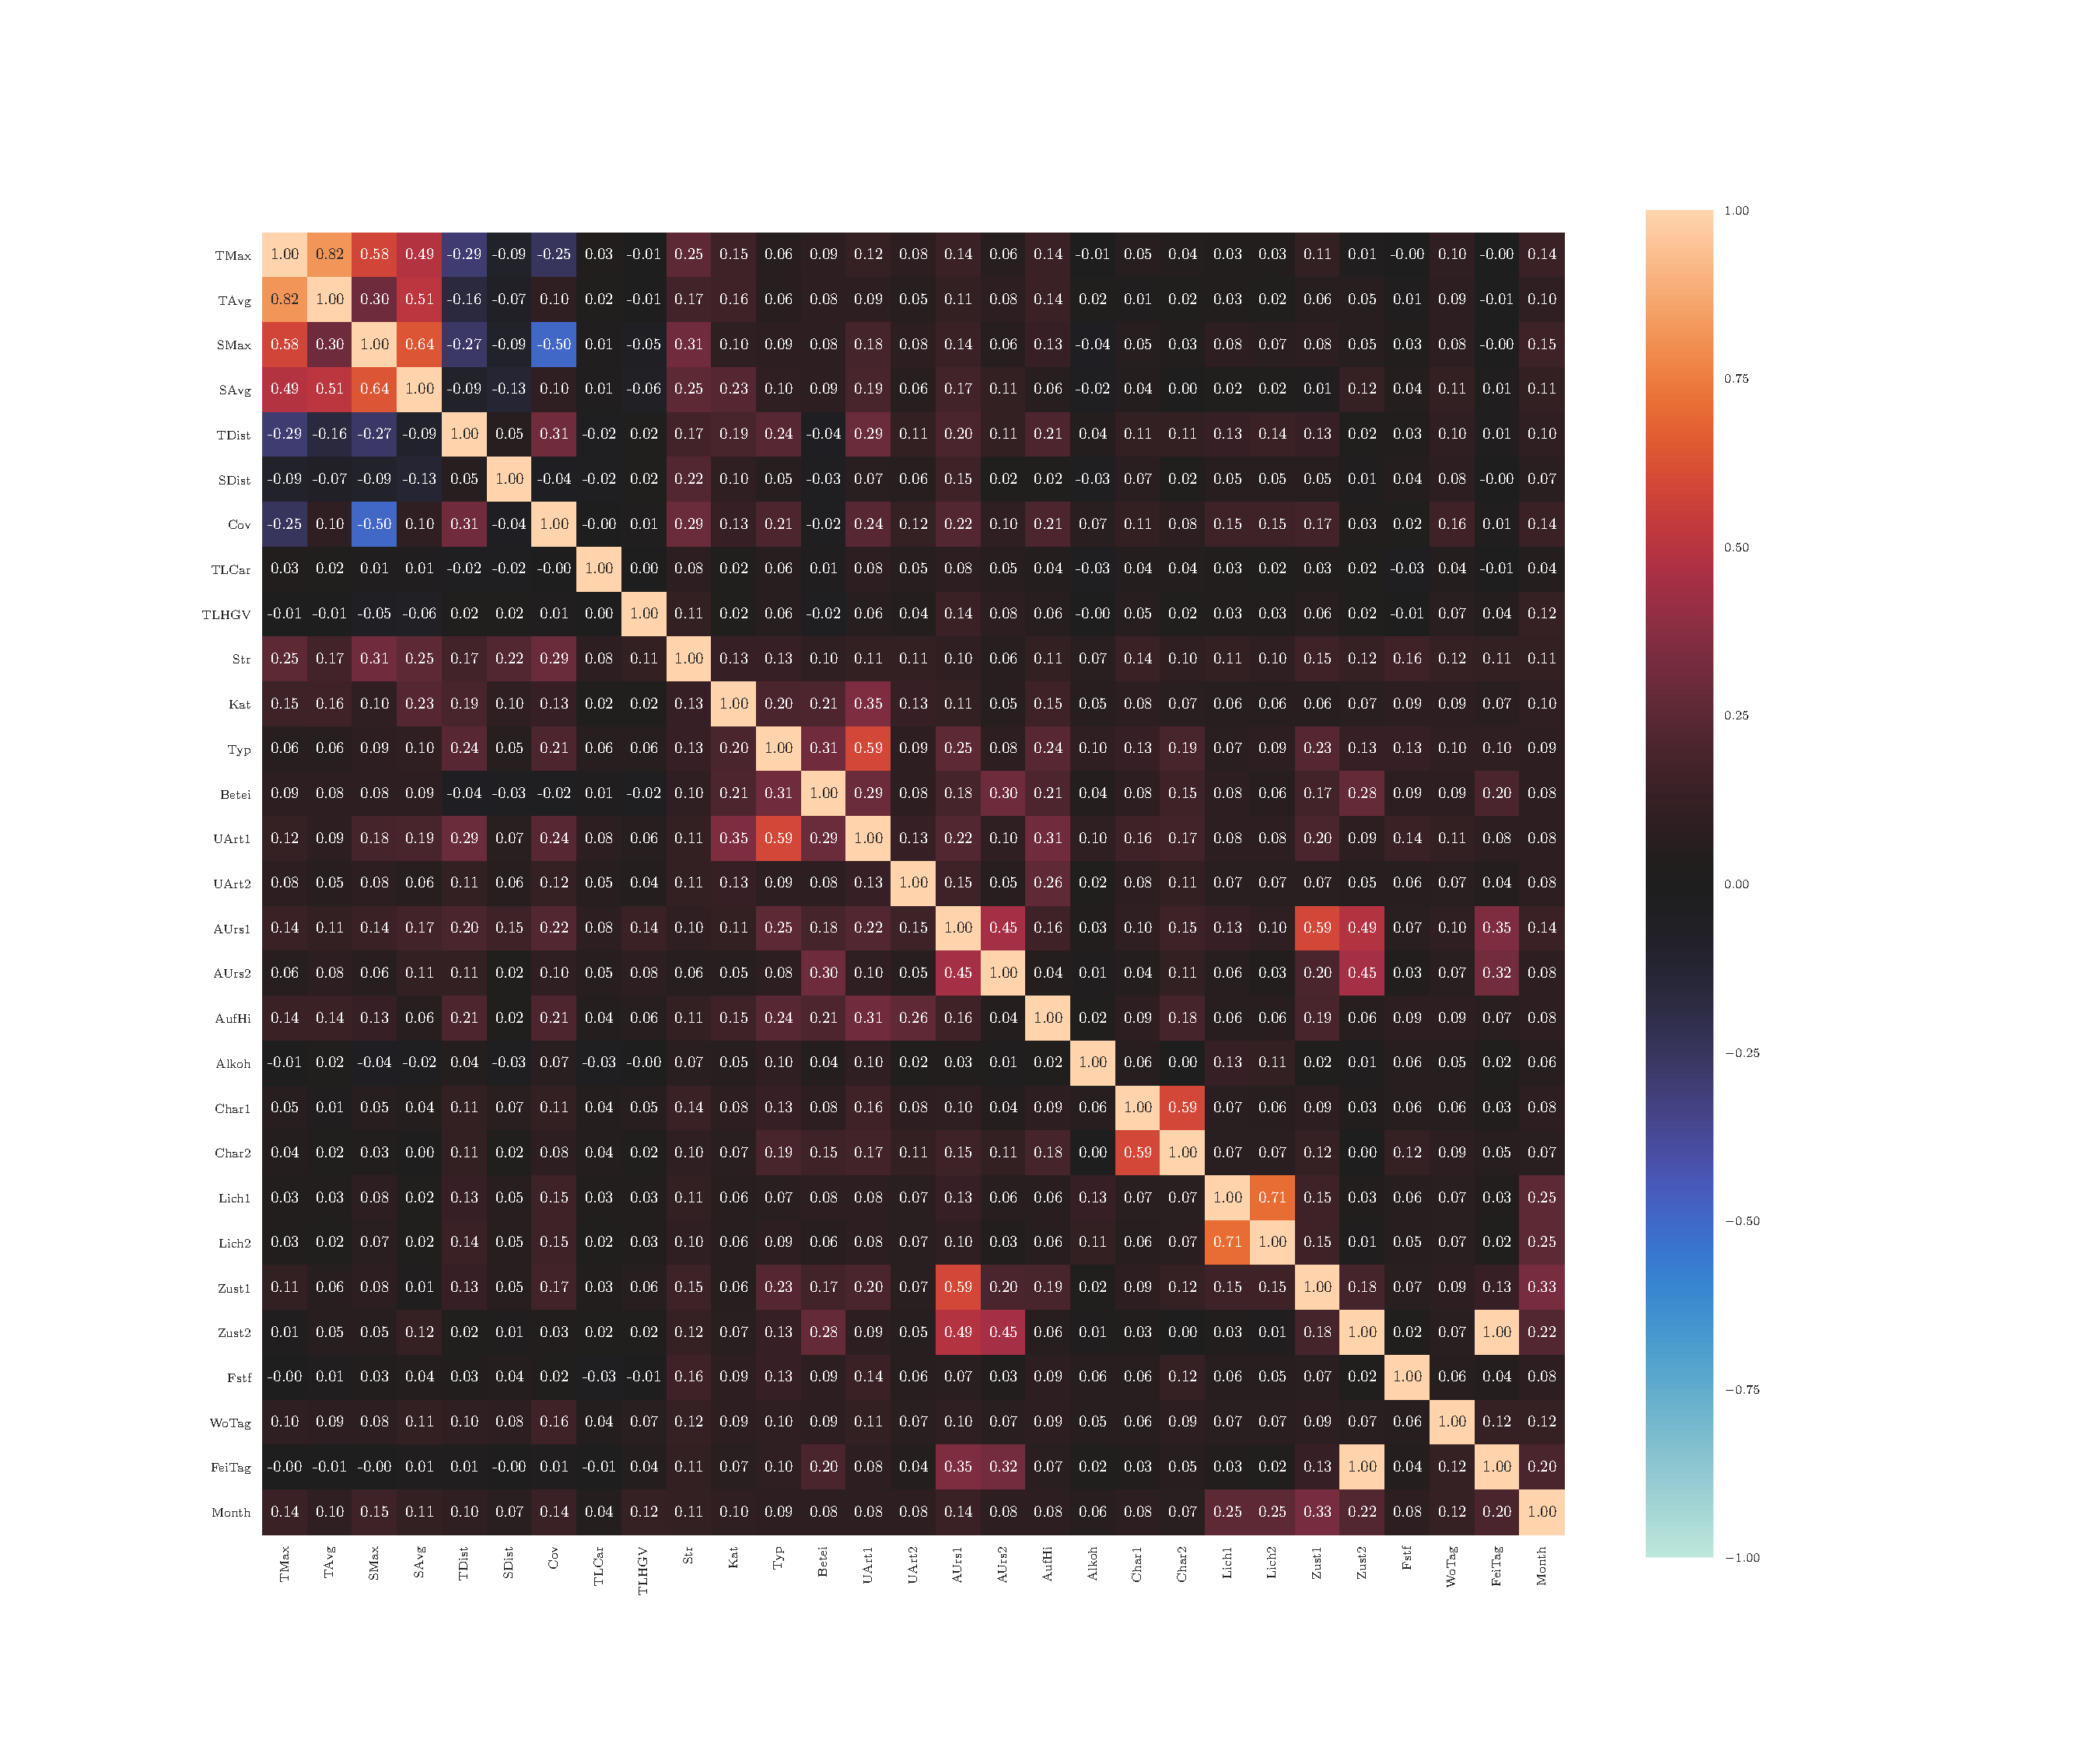
\includegraphics[width=1.4\textwidth, trim=0cm 2.5cm 6cm 3cm]{CorrAnalysis/data/BAYSIS/02_matched/plots/baysis_matched_corr_cramers}%
	}
	\caption{Correlation matrix for congestion-accident matched data, with $V$, $\eta$, $\tau$, $r_{pq}$, $r$}
	\label{img:correlation_matrix_matched_cramers}
\end{figure}

% --------------------------
% -------- Strasse ---------
% --------------------------
\centerheading{Strasse}
This section analyzes the correlated relations of the accident variable \textbf{Strasse}. The correlations of \textbf{Strasse}-\textbf{TDist} and \textbf{Strasse}-\textbf{SDist} produces a $p$-value above the $\alpha$-level of .05 in the Kruskal-Wallis rank sum test. The null hypothesis can't therefore be rejected for these relations and there are no significant groups to identify.

The Kruskal-Wallis rank sum test of \textbf{Strasse}-\textbf{TMax} produces a $p$-value of 0.000006, which is below $\alpha=.05$. The null hypothesis can therefore be rejected, which means there is a significant difference between the groups of \textbf{Strasse}. To identify the significant groups, a pairwise Wilcoxon $T$-test for \textbf{Strasse}-\textbf{TMax} is run, which produces \cref{tbl:wilcoxon_baysis_matched_Strasse_TMax}. 
\begin{table}[ht!]
	\tiny
	\setlength{\tabcolsep}{4pt}
	\centering
	\begin{tabular}{rrrrrrrrrrrrrrrrr}
		\toprule
				& A3 & A6 & A9 & A70 & A96 & A7 & A73 & A99 & A92 & A93 & A94 & A72 & A995 & A95 & A71 & A45 \\ 
		\midrule
		A6 		& 0.00 &  &  &  &  &  &  &  &  &  &  &  &  &  &  &  \\ 
		A9 		& 0.01 & 1.00 &  &  &  &  &  &  &  &  &  &  &  &  &  &  \\ 
		A70 	& 0.03 & 1.00 & 1.00 &  &  &  &  &  &  &  &  &  &  &  &  &  \\ 
		A96 	& 0.00 & 1.00 & 0.27 & 1.00 &  &  &  &  &  &  &  &  &  &  &  &  \\ 
		A7 		& 0.00 & 1.00 & 1.00 & 1.00 & 1.00 &  &  &  &  &  &  &  &  &  &  &  \\ 
		A73 	& 0.00 & 1.00 & 0.31 & 1.00 & 1.00 & 1.00 &  &  &  &  &  &  &  &  &  &  \\ 
		A99 	& 1.00 & 1.00 & 1.00 & 1.00 & 0.50 & 1.00 & 0.59 &  &  &  &  &  &  &  &  &  \\ 
		A92 	& 0.00 & 1.00 & 0.16 & 1.00 & 1.00 & 1.00 & 1.00 & 0.22 &  &  &  &  &  &  &  &  \\ 
		A93 	& 1.00 & 1.00 & 1.00 & 1.00 & 1.00 & 1.00 & 1.00 & 1.00 & 1.00 &  &  &  &  &  &  &  \\ 
		A94 	& 0.01 & 1.00 & 1.00 & 1.00 & 1.00 & 1.00 & 1.00 & 1.00 & 1.00 & 1.00 &  &  &  &  &  &  \\ 
		A72 	& 1.00 & 1.00 & 1.00 & 1.00 & 1.00 & 1.00 & 1.00 & 1.00 & 1.00 & 1.00 & 1.00 &  &  &  &  &  \\ 
		A995 	& 1.00 & 1.00 & 1.00 & 1.00 & 1.00 & 1.00 & 1.00 & 1.00 & 1.00 & 1.00 & 1.00 & 1.00 &  &  &  &  \\ 
		A95 	& 1.00 & 1.00 & 1.00 & 1.00 & 1.00 & 1.00 & 1.00 & 1.00 & 1.00 & 1.00 & 1.00 & 1.00 & 1.00 &  &  &  \\ 
		A71 	& 1.00 & 1.00 & 1.00 & 1.00 & 1.00 & 1.00 & 1.00 & 1.00 & 1.00 & 1.00 & 1.00 & 1.00 & 1.00 & 1.00 &  &  \\ 
		A45 	& 1.00 & 1.00 & 1.00 & 1.00 & 1.00 & 1.00 & 1.00 & 1.00 & 1.00 & 1.00 & 1.00 & 1.00 & 1.00 & 1.00 & 1.00 &  \\ 
		A980 	& 1.00 & 1.00 & 1.00 & 1.00 & 1.00 & 1.00 & 1.00 & 1.00 & 1.00 & 1.00 & 1.00 & 1.00 & 1.00 & 1.00 & 1.00 & 1.00 \\ 
		\bottomrule
	\end{tabular}
	\caption{Pairwise Wilcoxon $T$-test for \textit{Strasse} and \textit{Maximal Temporal Extent}}
	\label{tbl:wilcoxon_baysis_matched_Strasse_TMax}
\end{table}
\cref{tbl:wilcoxon_baysis_matched_Strasse_TMax} shows, that the groups A6, A9, A7, A70, A73, A92, A94 and A96 differ from group A3. There is no distinctive general trend.
\begin{table}[ht!]
	\tiny
	\centering
	\begin{tabular}{c|c|c|c|c|c|c|c}
		\toprule
		Group & $n$ & $\bar{x}$ & $\sigma$ & $\tilde{x}$ & $min$ & $max$ & $\Delta$ \\ 
		\midrule
		A3  & 559 & 225.76 & 210.36 & 156.00 & 9  & 1323 & 1314 \\ 
		A6  & 127 & 153.05 & 150.42 & 108.00 & 12 & 864  & 852  \\ 
		A9  & 466 & 170.85 & 151.33 & 118.50 & 9  & 1194 & 1185 \\ 
		A70 & 31  & 106.55 & 79.42  & 81.00  & 24 & 369  & 345  \\ 
		A96 & 155 & 118.32 & 81.05  & 108.00 & 12 & 384  & 372  \\ 
		A7  & 130 & 153.37 & 194.10 & 102.00 & 9  & 1341 & 1332 \\ 
		A73 & 129 & 125.95 & 135.01 & 93.00  & 12 & 1323 & 1311 \\ 
		A99 & 116 & 169.09 & 136.72 & 138.00 & 15 & 681  & 666  \\ 
		A92 & 66  & 103.86 & 65.69  & 87.00  & 18 & 354  & 336  \\ 
		A93 & 21  & 163.57 & 155.71 & 111.00 & 36 & 588  & 552  \\ 
		A94 & 37  & 101.59 & 54.60  & 99.00  & 15 & 249  & 234  \\ 
 		\bottomrule
	\end{tabular}
	\caption{Group descriptives of \textit{Strasse} and \textit{Maximal Temporal Extent}}
	\label{tbl:descriptives_baysis_matched_Strasse_TMax}
	%\vspace{-8mm}
\end{table}
The descriptives from \cref{tbl:descriptives_baysis_matched_Strasse_TMax} show that the mean value of A3 is 27\,\% - 57\,\% higher than the means of A6, A7, A9, A70, A73, A92, and A94. It can be interpreted that accidents on the A3 are associated with significantly longer (temporal) jams than on the A6, A9, A7, A70, A73, A92, and A94.

The Kruskal-Wallis rank sum test of \textbf{Strasse}-\textbf{TAvg} produces a $p$-value of 0.000466, which is below $\alpha=.05$. The null hypothesis can therefore be rejected, which means there is a significant difference between the groups of \textbf{Strasse}. To identify the significant groups, a pairwise Wilcoxon $T$-test for \textbf{Strasse}-\textbf{TAvg} is run, which produces \cref{tbl:wilcoxon_baysis_matched_Strasse_TAvg}. 
\begin{table}[ht!]
	\tiny
	\setlength{\tabcolsep}{4pt}
	\centering
	\begin{tabular}{rrrrrrrrrrrrrrrrr}
		\toprule
				& A3 & A6 & A9 & A70 & A96 & A7 & A73 & A99 & A92 & A93 & A94 & A72 & A995 & A95 & A71 & A45 \\ 
		\midrule
		A6 		& 0.84 &  &  &  &  &  &  &  &  &  &  &  &  &  &  &  \\ 
		A9 		& 0.36 & 1.00 &  &  &  &  &  &  &  &  &  &  &  &  &  &  \\ 
		A70		& 1.00 & 1.00 & 1.00 &  &  &  &  &  &  &  &  &  &  &  &  &  \\ 
		A96 	& 0.10 & 1.00 & 1.00 & 1.00 &  &  &  &  &  &  &  &  &  &  &  &  \\ 
		A7 		& 1.00 & 1.00 & 1.00 & 1.00 & 1.00 &  &  &  &  &  &  &  &  &  &  &  \\ 
		A73 	& 0.00 & 1.00 & 0.51 & 1.00 & 1.00 & 1.00 &  &  &  &  &  &  &  &  &  &  \\ 
		A99 	& 0.02 & 1.00 & 1.00 & 1.00 & 1.00 & 1.00 & 1.00 &  &  &  &  &  &  &  &  &  \\ 
		A92 	& 0.26 & 1.00 & 1.00 & 1.00 & 1.00 & 1.00 & 1.00 & 1.00 &  &  &  &  &  &  &  &  \\ 
		A93 	& 1.00 & 1.00 & 1.00 & 1.00 & 1.00 & 1.00 & 1.00 & 1.00 & 1.00 &  &  &  &  &  &  &  \\ 
		A94 	& 0.28 & 1.00 & 1.00 & 1.00 & 1.00 & 1.00 & 1.00 & 1.00 & 1.00 & 1.00 &  &  &  &  &  &  \\ 
		A72 	& 1.00 & 1.00 & 1.00 & 1.00 & 1.00 & 1.00 & 1.00 & 1.00 & 1.00 & 1.00 & 1.00 &  &  &  &  &  \\ 
		A995 	& 1.00 & 1.00 & 1.00 & 1.00 & 1.00 & 1.00 & 1.00 & 1.00 & 1.00 & 1.00 & 1.00 & 1.00 &  &  &  &  \\ 
		A95 	& 1.00 & 1.00 & 1.00 & 1.00 & 1.00 & 1.00 & 1.00 & 1.00 & 1.00 & 1.00 & 1.00 & 1.00 & 1.00 &  &  &  \\ 
		A71		& 1.00 & 1.00 & 1.00 & 1.00 & 1.00 & 1.00 & 1.00 & 1.00 & 1.00 & 1.00 & 1.00 & 1.00 & 1.00 & 1.00 &  &  \\ 
		A45 	& 1.00 & 1.00 & 1.00 & 1.00 & 1.00 & 1.00 & 1.00 & 1.00 & 1.00 & 1.00 & 1.00 & 1.00 & 1.00 & 1.00 & 1.00 &  \\ 
		A980 	& 1.00 & 1.00 & 1.00 & 1.00 & 1.00 & 1.00 & 1.00 & 1.00 & 1.00 & 1.00 & 1.00 & 1.00 & 1.00 & 1.00 & 1.00 & 1.00 \\
		\bottomrule
	\end{tabular}
	\caption{Pairwise Wilcoxon $T$-test for \textit{Strasse} and \textit{Average Temporal Extent}}
	\label{tbl:wilcoxon_baysis_matched_Strasse_TAvg}
\end{table}
\cref{tbl:wilcoxon_baysis_matched_Strasse_TAvg} shows, that the groups A73, A99 and A96 differ from group A3. There is no distinctive general trend.
\begin{table}[ht!]
	\tiny
	\centering
	\begin{tabular}{c|c|c|c|c|c|c|c}
		\toprule
		Group & $n$ & $\bar{x}$ & $\sigma$ & $\tilde{x}$ & $min$ & $max$ & $\Delta$ \\  
		\midrule
		A3  & 559 & 89.66 & 98.94  & 65.00 & 4  & 1260 & 1256 \\ 
		A6  & 127 & 69.94 & 65.86  & 56.00 & 3  & 376  & 373  \\ 
		A9  & 466 & 72.92 & 64.55  & 54.00 & 4  & 575  & 571  \\ 
		A70 & 31  & 50.10 & 23.99  & 49.00 & 10 & 99   & 89   \\ 
		A96 & 155 & 61.37 & 44.31  & 52.50 & 5  & 247  & 242  \\ 
		A7  & 130 & 86.55 & 146.82 & 59.50 & 6  & 1326 & 1320 \\ 
		A73 & 129 & 54.78 & 42.48  & 45.00 & 6  & 274  & 268  \\ 
		A99 & 116 & 58.97 & 48.35  & 47.50 & 4  & 295  & 291  \\ 
		A92 & 66  & 55.24 & 36.43  & 51.50 & 8  & 235  & 227  \\ 
		A93 & 21  & 82.33 & 91.10  & 48.00 & 7  & 343  & 336  \\ 
		A94 & 37  & 49.86 & 31.63  & 44.00 & 14 & 145  & 131  \\ 
		\bottomrule
	\end{tabular}
	\caption{Group descriptives for \textit{Strasse} and \textit{Average Temporal Extent}}
	\label{tbl:descriptives_baysis_matched_Strasse_TAvg}
	%\vspace{-8mm}
\end{table}
The descriptives from \cref{tbl:descriptives_baysis_matched_Strasse_TAvg} show that the mean value of A3 is about $\frac{1}{3}$ higher than the means of A73, A99 and A96. We can interpret that accidents on the A3 are associated with significantly longer (temporal) jams than on A73, A99 and A96.

The Kruskal-Wallis rank sum test of \textbf{Strasse}-\textbf{SMax} produces a $p$-value of 0.000003, which is below $\alpha=.05$. The null hypothesis can therefore be rejected, which means there is a significant difference between the groups of \textbf{Strasse}. To identify the significant groups, a pairwise Wilcoxon $T$-test for \textbf{Strasse}-\textbf{SMax} is run, which produces \cref{tbl:wilcoxon_baysis_matched_Strasse_SMax}.
\begin{table}[ht!]
	\tiny
	\setlength{\tabcolsep}{4pt}
	\centering
	\begin{tabular}{rrrrrrrrrrrrrrrrr}
		\toprule
				& A3   & A6   & A9   & A70  & A96  & A7   & A73   & A99 & A92 & A93 & A94 & A72 & A995 & A95 & A71 & A45 \\ 
		\midrule
		A6 		& 0.40 &  &  &  &  &  &  &  &  &  &  &  &  &  &  &  \\ 
		A9 		& 0.00 & 1.00 &  &  &  &  &  &  &  &  &  &  &  &  &  &  \\ 
		A70 	& 0.00 & 0.83 & 0.54 &  &  &  &  &  &  &  &  &  &  &  &  &  \\ 
		A96 	& 0.00 & 1.00 & 0.14 & 1.00 &  &  &  &  &  &  &  &  &  &  &  &  \\ 
		A7 		& 0.00 & 1.00 & 1.00 & 1.00 & 1.00 &  &  &  &  &  &  &  &  &  &  &  \\ 
		A73 	& 0.00 & 0.00 & 0.00 & 1.00 & 1.00 & 0.59 &  &  &  &  &  &  &  &  &  &  \\ 
		A99 	& 1.00 & 1.00 & 1.00 & 0.80 & 0.31 & 1.00 & 0.00 &  &  &  &  &  &  &  &  &  \\ 
		A92 	& 0.00 & 0.00 & 0.00 & 1.00 & 1.00 & 1.00 & 1.00 & 0.00 &  &  &  &  &  &  &  &  \\ 
		A93 	& 0.03 & 1.00 & 1.00 & 1.00 & 1.00 & 1.00 & 1.00 & 1.00 & 1.00 &  &  &  &  &  &  &  \\ 
		A94 	& 0.00 & 0.11 & 0.03 & 1.00 & 1.00 & 1.00 & 1.00 & 0.09 & 1.00 & 1.00 &  &  &  &  &  &  \\ 
		A72 	& 1.00 & 1.00 & 1.00 & 1.00 & 1.00 & 1.00 & 1.00 & 1.00 & 1.00 & 1.00 & 1.00 &  &  &  &  &  \\ 
		A995 	& 1.00 & 1.00 & 1.00 & 1.00 & 1.00 & 1.00 & 1.00 & 1.00 & 1.00 & 1.00 & 1.00 & 1.00 &  &  &  &  \\ 
		A95 	& 1.00 & 1.00 & 1.00 & 1.00 & 1.00 & 1.00 & 1.00 & 1.00 & 1.00 & 1.00 & 1.00 & 1.00 & 1.00 &  &  &  \\ 
		A71 	& 1.00 & 1.00 & 1.00 & 1.00 & 1.00 & 1.00 & 1.00 & 1.00 & 1.00 & 1.00 & 1.00 & 1.00 & 1.00 & 1.00 &  &  \\ 
		A45 	& 1.00 & 1.00 & 1.00 & 1.00 & 1.00 & 1.00 & 1.00 & 1.00 & 1.00 & 1.00 & 1.00 & 1.00 & 1.00 & 1.00 & 1.00 &  \\ 
		A980 	& 1.00 & 1.00 & 1.00 & 1.00 & 1.00 & 1.00 & 1.00 & 1.00 & 1.00 & 1.00 & 1.00 & 1.00 & 1.00 & 1.00 & 1.00 & 1.00 \\ 
		\bottomrule
	\end{tabular}
	\caption{Pairwise Wilcoxon $T$-test for \textit{Strasse} and \textit{Maximal Spatial Extent}}
	\label{tbl:wilcoxon_baysis_matched_Strasse_SMax}
\end{table}
\cref{tbl:wilcoxon_baysis_matched_Strasse_SMax} shows, that the groups A7, A9, A70, A73, A92, A94 and A96 differ from group A3. The groups A73 and A92 further differ from group A6 and A9. The group A99 differs from group A73 and group A99 differs from A92. There is no distinctive general trend.
\begin{table}[ht!]
	\tiny
	\centering
	\begin{tabular}{c|c|c|c|c|c|c|c}
		\toprule
		Group & $n$ & $\bar{x}$ & $\sigma$ & $\tilde{x}$ & $min$ & $max$ & $\Delta$ \\  
		\midrule
		A3 & 574 & 17804.82 & 27554.53 & 11367.00 & 1084.00 & 219082.00 & 217998.00 \\ 
		A6 & 127 & 11067.98 & 8428.07 & 8634.00  & 965.00 & 43156.00 & 42191.00 \\ 
		A9 & 466 & 10680.48 & 7724.45 & 8977.50 & 832.00 & 49765.00 & 48933.00 \\ 
		A70 & 31 & 6676.39 & 3640.24 & 6136.00 & 1841.00 & 13058.00 & 11217.00 \\ 
		A96 & 156 & 8950.30 & 8116.21 & 6315.00 & 971.00 & 70726.00 & 69755.00 \\ 
		A7 & 130 & 9018.27 & 7293.14 & 7051.50 & 1108.00 & 43244.00 & 42136.00 \\ 
		A73 & 129 & 6502.88 & 5033.20 & 5327.00 & 1036.00 & 33764.00 & 32728.00 \\ 
		A99 & 116 & 13244.02 & 11313.27 & 9439.50 & 1280.00 & 48278.00 & 46998.00 \\ 
		A92 & 66 & 6186.80 & 4000.10 & 4936.50 & 1176.00 & 23291.00 & 22115.00 \\ 
		A93 & 21 & 6765.00 & 4403.32 & 5323.00 & 1244.00 & 16922.00 & 15678.00 \\ 
		A94 & 37 & 6220.38 & 3984.46 & 5768.00 & 1167.00 & 15550.00 & 14383.00 \\ 
		%A72 & 1 & 3952.00 &  & 3952.00 & 3952.00 & 3952.00 & 0.00 \\ 
		%A995 & 2 & 1866.50 & 133.64 & 1866.50 & 1772.00 & 1961.00 & 189.00 \\ 
		%A95 & 4 & 4995.75 & 1065.05 & 4925.50 & 3798.00 & 6334.00 & 2536.00 \\ 
		%A71 & 3 & 4890.33 & 3031.47 & 6342.00 & 1406.00 & 6923.00 & 5517.00 \\ 
		%A45 & 3 & 3693.00 & 3286.40 & 1864.00 & 1728.00 & 7487.00 & 5759.00 \\ 
		%A980 & 1 & 1925.00 &  & 1925.00 & 1925.00 & 1925.00 & 0.00 \\ 
		\bottomrule
	\end{tabular}
	\caption{Group descriptives of \textit{Strasse} and \textit{Maximal Spatial Extent}}
	\label{tbl:descriptives_baysis_matched_Strasse_SMax}
	%\vspace{-8mm}
\end{table}
The descriptives from \cref{tbl:descriptives_baysis_matched_Strasse_SMax} show that the mean of A3 is 44\,\% - 66\,\% higher than the means of A7, A9, A70, A73, A92, A94 and A96. It also shows that the groups A6, A9 and A99 have a up to 50\,\% higher mean than the groups A73 and A92. We can interpret that accidents on the A3, A6, A9 and A99 are associated with significantly longer (spatial) jams than on A7, A73, A92, A94 and A96.

The Kruskal-Wallis rank sum test of \textbf{Strasse}-\textbf{SAvg} produces a $p$-value of 0.002086, which is below $\alpha=.05$. The null hypothesis can therefore be rejected, which means there is a significant difference between the groups of \textbf{Strasse}. To identify the significant groups, a pairwise Wilcoxon $T$-test for \textbf{Strasse}-\textbf{SAvg} is run, which produces \cref{tbl:wilcoxon_baysis_matched_Strasse_SAvg}.
\begin{table}[ht!]
	\tiny
	\setlength{\tabcolsep}{4pt}
	\centering
	\begin{tabular}{rrrrrrrrrrrrrrrrr}
		\toprule
	 		 & A3 & A6 & A9 & A70 & A96 & A7 & A73 & A99 & A92 & A93 & A94 & A72 & A995 & A95 & A71 & A45 \\ 
		\midrule
		A6   & 1.00 &  &  &  &  &  &  &  &  &  &  &  &  &  &  &  \\ 
	  	A9   & 1.00 & 1.00 &  &  &  &  &  &  &  &  &  &  &  &  &  &  \\ 
	  	A70  & 0.03 & 0.83 & 0.71 &  &  &  &  &  &  &  &  &  &  &  &  &  \\ 
	  	A96  & 0.01 & 1.00 & 1.00 & 1.00 &  &  &  &  &  &  &  &  &  &  &  &  \\ 
	  	A7   & 1.00 & 1.00 & 1.00 & 1.00 & 1.00 &  &  &  &  &  &  &  &  &  &  &  \\ 
	  	A73  & 0.00 & 0.00 & 0.00 & 1.00 & 0.00 & 0.00 &  &  &  &  &  &  &  &  &  &  \\ 
	  	A99  & 0.00 & 1.00 & 0.06 & 1.00 & 1.00 & 1.00 & 0.51 &  &  &  &  &  &  &  &  &  \\ 
	  	A92  & 0.00 & 0.61 & 0.03 & 1.00 & 1.00 & 1.00 & 1.00 & 1.00 &  &  &  &  &  &  &  &  \\ 
	  	A93  & 0.02 & 0.46 & 0.16 & 1.00 & 1.00 & 1.00 & 1.00 & 1.00 & 1.00 &  &  &  &  &  &  &  \\ 
	  	A94  & 0.00 & 0.07 & 0.01 & 1.00 & 0.36 & 0.31 & 1.00 & 1.00 & 1.00 & 1.00 &  &  &  &  &  &  \\ 
	  	A72  & 1.00 & 1.00 & 1.00 & 1.00 & 1.00 & 1.00 & 1.00 & 1.00 & 1.00 & 1.00 & 1.00 &  &  &  &  &  \\ 
	  	A995 & 1.00 & 1.00 & 1.00 & 1.00 & 1.00 & 1.00 & 1.00 & 1.00 & 1.00 & 1.00 & 1.00 & 1.00 &  &  &  &  \\ 
	  	A95  & 1.00 & 1.00 & 1.00 & 1.00 & 1.00 & 1.00 & 1.00 & 1.00 & 1.00 & 1.00 & 1.00 & 1.00 & 1.00 &  &  &  \\ 
	  	A71  & 1.00 & 1.00 & 1.00 & 1.00 & 1.00 & 1.00 & 1.00 & 1.00 & 1.00 & 1.00 & 1.00 & 1.00 & 1.00 & 1.00 &  &  \\ 
	  	A45  & 1.00 & 1.00 & 1.00 & 1.00 & 1.00 & 1.00 & 1.00 & 1.00 & 1.00 & 1.00 & 1.00 & 1.00 & 1.00 & 1.00 & 1.00 &  \\ 
	  	A980 & 1.00 & 1.00 & 1.00 & 1.00 & 1.00 & 1.00 & 1.00 & 1.00 & 1.00 & 1.00 & 1.00 & 1.00 & 1.00 & 1.00 & 1.00 & 1.00 \\ 
		\bottomrule
	\end{tabular}
	\caption{Pairwise Wilcoxon $T$-test for \textit{Strasse} and \textit{Average Spatial Extent}}
	\label{tbl:wilcoxon_baysis_matched_Strasse_SAvg}
\end{table}
\cref{tbl:wilcoxon_baysis_matched_Strasse_SAvg} shows, that the groups A70, A73, A92, A93, A94, A96 and A99 differ from group A3. The groups A73, A94 further differ from group A6 as well as A73, A99, A92 and A94 from group A9. There is no distinctive general trend.
\begin{table}[ht!]
	\tiny
	\centering
	\begin{tabular}{c|c|c|c|c|c|c|c}
	  	\toprule
	 	Group & $n$ & $\bar{x}$ & $\sigma$ & $\tilde{x}$ & $min$ & $max$ & $\Delta$ \\  
	  	\midrule
		A3 & 574.00 & 4624.11 & 2781.72 & 4035.50 & 135.00 & 17805.00 & 17670.00 \\ 
	  	A6 & 127.00 & 4361.50 & 3042.71 & 3235.00 & 458.00 & 16851.00 & 16393.00 \\ 
	  	A9 & 466.00 & 4187.15 & 2569.83 & 3700.50 & 393.00 & 15132.00 & 14739.00 \\ 
	  	A70 & 31.00 & 3010.45 & 2067.63 & 1974.00 & 1008.00 & 9937.00 & 8929.00 \\ 
	  	A96 & 156.00 & 3664.63 & 2172.78 & 3292.50 & 387.00 & 10182.00 & 9795.00 \\ 
	  	A7 & 130.00 & 4141.68 & 3026.58 & 3537.50 & 643.00 & 16571.00 & 15928.00 \\ 
	  	A73 & 129.00 & 2683.97 & 1981.91 & 2232.00 & 544.00 & 11832.00 & 11288.00 \\ 
	  	A99 & 116.00 & 3240.97 & 1878.87 & 2978.00 & 583.00 & 8426.00 & 7843.00 \\ 
	  	A92 & 66.00 & 2926.15 & 1521.59 & 2931.50 & 455.00 & 8970.00 & 8515.00 \\ 
	  	A93 & 21.00 & 2525.43 & 1443.21 & 2338.00 & 664.00 & 6779.00 & 6115.00 \\ 
	  	A94 & 37.00 & 2691.68 & 2023.38 & 2307.00 & 358.00 & 10393.00 & 10035.00 \\ 
	   	\bottomrule
	\end{tabular}
	\caption{Group descriptives of \textit{Strasse} and \textit{Average Spatial Extent}}
	\label{tbl:descriptives_baysis_matched_Strasse_SAvg}
	%\vspace{-8mm}
\end{table}
The descriptives from \cref{tbl:descriptives_baysis_matched_Strasse_SAvg} show that the mean of A3 is 45\,\% - 55\,\% higher the means of A70, A73, A92, A93, A94, A96 and A99. It also shows that the means of the groups A6, A9 and A99 is about 30\,\% higher mean than the groups A73 and A94. We can interpret that accidents on the A3, A6, A9 and A99 lead are associated with significantly longer (spatial) jams than on A70, A73, A92, A93, A94, A96 and A99.

The Kruskal-Wallis rank sum test of \textbf{Strasse}-\textbf{Cov} produces a $p$-value of 0.000317, which is below $\alpha=.05$. The null hypothesis can therefore be rejected, which means there is a significant difference between the groups of \textbf{Strasse}. To identify the significant groups, a pairwise Wilcoxon $T$-test for \textbf{Strasse}-\textbf{Cov} is run, which produces \cref{tbl:wilcoxon_baysis_matched_Strasse_Cov}. 
\begin{table}[ht!]
	\tiny
	\setlength{\tabcolsep}{4pt}
	\centering
	\begin{tabular}{rrrrrrrrrrrrrrrrr}
	  	\toprule
				& A3   & A6   & A9   & A70  & A96  & A7   & A73 & A99 & A92 & A93 & A94 & A72 & A995 & A95 & A71 & A45 \\ 
	  	\midrule
		A6 		& 0.01 &  &  &  &  &  &  &  &  &  &  &  &  &  &  &  \\ 
	  	A9 		& 0.00 & 1.00 &  &  &  &  &  &  &  &  &  &  &  &  &  &  \\ 
	  	A70 	& 0.74 & 1.00 & 1.00 &  &  &  &  &  &  &  &  &  &  &  &  &  \\ 
	  	A96 	& 0.00 & 1.00 & 0.00 & 1.00 &  &  &  &  &  &  &  &  &  &  &  &  \\ 
	  	A7 		& 0.00 & 1.00 & 0.01 & 1.00 & 1.00 &  &  &  &  &  &  &  &  &  &  &  \\ 
	  	A73 	& 0.01 & 1.00 & 1.00 & 1.00 & 1.00 & 1.00 &  &  &  &  &  &  &  &  &  &  \\ 
	  	A99 	& 1.00 & 0.00 & 0.00 & 0.09 & 0.00 & 0.00 & 0.00 &  &  &  &  &  &  &  &  &  \\ 
	  	A92 	& 0.00 & 1.00 & 0.12 & 1.00 & 1.00 & 1.00 & 1.00 & 0.00 &  &  &  &  &  &  &  &  \\ 
	  	A93 	& 1.00 & 1.00 & 1.00 & 1.00 & 1.00 & 1.00 & 1.00 & 1.00 & 1.00 &  &  &  &  &  &  &  \\ 
	  	A94 	& 1.00 & 1.00 & 1.00 & 1.00 & 1.00 & 1.00 & 1.00 & 0.13 & 1.00 & 1.00 &  &  &  &  &  &  \\ 
	  	A72 	& 1.00 & 1.00 & 1.00 & 1.00 & 1.00 & 1.00 & 1.00 & 1.00 & 1.00 & 1.00 & 1.00 &  &  &  &  &  \\ 
	  	A995 	& 1.00 & 1.00 & 1.00 & 1.00 & 1.00 & 1.00 & 1.00 & 1.00 & 1.00 & 1.00 & 1.00 & 1.00 &  &  &  &  \\ 
	  	A95 	& 1.00 & 1.00 & 1.00 & 1.00 & 1.00 & 1.00 & 1.00 & 1.00 & 1.00 & 1.00 & 1.00 & 1.00 & 1.00 &  &  &  \\ 
	  	A71 	& 1.00 & 1.00 & 1.00 & 1.00 & 1.00 & 1.00 & 1.00 & 1.00 & 1.00 & 1.00 & 1.00 & 1.00 & 1.00 & 1.00 &  &  \\ 
	  	A45 	& 1.00 & 1.00 & 1.00 & 1.00 & 1.00 & 1.00 & 1.00 & 1.00 & 1.00 & 1.00 & 1.00 & 1.00 & 1.00 & 1.00 & 1.00 &  \\ 
	  	A980 	& 1.00 & 1.00 & 1.00 & 1.00 & 1.00 & 1.00 & 1.00 & 1.00 & 1.00 & 1.00 & 1.00 & 1.00 & 1.00 & 1.00 & 1.00 & 1.00 \\ 
	   	\bottomrule
	\end{tabular}
	\caption{Pairwise Wilcoxon $T$-test for \textit{Street} and \textit{Coverage}}
	\label{tbl:wilcoxon_baysis_matched_Strasse_Cov}
\end{table}
\cref{tbl:wilcoxon_baysis_matched_Strasse_SAvg} shows, that the groups A6, A7, A9, A73, A92 and A96 differ from group A3. The group A99 differs from group A6 and groups A96, AA7, A99, A92 differ from group A9. The group A99 also differs from the groups A70, A96, A7 and A73. There is no distinctive general trend. 
\begin{table}[ht!]
	\tiny
	\centering
	\begin{tabular}{c|c|c|c|c|c|c|c}
	  	\toprule
	 	Group & $n$ & $\bar{x}$ & $\sigma$ & $\tilde{x}$ & $min$ & $max$ & $\Delta$ \\   
	  	\midrule
		A3 & 574.00 & 37.59 & 19.51 & 35.00 & 2.00 & 100.00 & 98.00 \\ 
	  	A6 & 127.00 & 46.99 & 24.06 & 44.00 & 9.00 & 100.00 & 91.00 \\ 
	  	A9 & 466.00 & 43.93 & 18.49 & 41.00 & 6.00 & 100.00 & 94.00 \\ 
	  	A70 & 31.00 & 50.29 & 25.00 & 44.00 & 9.00 & 92.00 & 83.00 \\ 
	  	A96 & 156.00 & 51.62 & 21.68 & 54.00 & 2.00 & 100.00 & 98.00 \\ 
	  	A7 & 130.00 & 53.46 & 24.19 & 54.00 & 6.00 & 100.00 & 94.00 \\ 
	  	A73 & 129.00 & 46.49 & 22.88 & 42.00 & 7.00 & 100.00 & 93.00 \\ 
	  	A99 & 116.00 & 33.21 & 18.03 & 31.00 & 5.00 & 85.00 & 80.00 \\ 
	  	A92 & 66.00 & 53.15 & 21.80 & 52.50 & 14.00 & 98.00 & 84.00 \\ 
	  	A93 & 21.00 & 40.81 & 17.72 & 37.00 & 13.00 & 70.00 & 57.00 \\ 
	  	A94 & 37.00 & 47.76 & 23.69 & 44.00 & 11.00 & 88.00 & 77.00 \\ 	
	  	\bottomrule
	\end{tabular}
	\caption{Group descriptives of \textit{Strasse} and \textit{Coverage}}
	\label{tbl:descriptives_baysis_matched_Strasse_Cov}
	%\vspace{-8mm}
\end{table}
The descriptives from \cref{tbl:descriptives_baysis_matched_Strasse_Cov} show that the mean of A3 is 20\,\% - 30\,\% lower than the means of A6, A7, A9, A73, A92 and A96. It also shows that the mean of A6 is about $\frac{1}{3}$ higher than the mean of A99. We can interpret that accidents on the A3, A99 are associated with significantly less denser jams than on A6, A7, A9, A73, A70, A92 and A96.

% ----------------------
% -------- Kat ---------
% ----------------------
\centerheading{Kat}
This section analyzes the correlated relations of the accident variable \textbf{Kat} and introduces a initial interpretation of each significant correlation. Groups with an insufficient sample size (see \cref{correlation_uncertainty} are neglected and not considered. The encoding and description of the variable \textbf{Typ} is shown in \cref{tbl:baysis_dataset_Typ}. The Kruskal-Wallis rank sum test of \textbf{Kat}-\textbf{SAvg} produces a $p$-value above $\alpha=.05$. The null hypothesis can't be rejected and there is no significant difference between the groups of \textbf{Kat} in this relation.

The Kruskal-Wallis rank sum test of \textbf{Kat}-\textbf{TMax} produces a $p$-value of 0.00682, which is below $\alpha=.05$. The null hypothesis can therefore be rejected, which means there is a significant difference between the groups of \textbf{Kat}. To identify the significant groups, a pairwise Wilcoxon $T$-test for \textbf{Kat}-\textbf{TMax} is run, which produces \cref{tbl:wilcoxon_baysis_matched_Kat_TMax}.
\begin{table}[ht]
	\small
	\centering
	\begin{tabular}{rrrr}
	  	\toprule
	 	& 1 & 2 & 3 \\ 
	  	\midrule
		2 & 0.00 &  &  \\ 
	  	3 & 0.00 & 0.01 &  \\ 
	  	7 & 0.00 & 0.02 & 0.78 \\ 
	   	\bottomrule
	\end{tabular}
	\caption{Pairwise Wilcoxon $T$-test for \textit{Kat} and \textit{Maximal Temporal Extent}}
	\label{tbl:wilcoxon_baysis_matched_Kat_TMax}
\end{table}
\cref{tbl:wilcoxon_baysis_matched_Kat_TMax} shows that all groups, besides of group 7 to group 3, have significant differences. 
\begin{table}[ht]
	\small
	\centering
	\begin{tabular}{c|c|c|c|c|c|c|c}
		\toprule
		Group & $n$ & $\bar{x}$ & $\sigma$ & $\tilde{x}$ & $min$ & $max$ & $\Delta$ \\   
	  	\midrule
		1 & 36.00 & 317.67 & 215.10 & 279.00   & 27.00 & 987.00 & 960.00  \\ 
	  	2 & 216.00 & 189.03 & 164.93 & 135.00 & 9.00 & 1257.00 & 1248.00  \\ 
	  	3 & 881.00 & 155.26 & 141.87 & 111.00 & 9.00 & 1323.00 & 1314.00  \\ 
	  	7 & 718.00 & 179.35 & 192.33 & 117.00  & 9.00 & 1341.00 & 1332.00 \\ 
	   	\bottomrule
	\end{tabular}
	\caption{Group descriptives of \textit{Kat} and \textit{Maximal Temporal Extent}}
	\label{tbl:descriptives_baysis_matched_Kat_TMax}
	%\vspace{-8mm}
\end{table}
The descriptives from \cref{tbl:descriptives_baysis_matched_Kat_TMax} present increasing means from lightly injured to deathly accident. We can interpret that the maximal jam length (temporal) increases with the gravity of the accident. Also the difference of group 1 to group 2 is quite substantial, which means that the accidents with deaths are associated with 40\,\% longer jams, than others. The group of accidents with property damage does significantly differ from the others. A comparisons of means puts the group in-between of accidents with slightly and heavily injured.

The Kruskal-Wallis rank sum test of \textbf{Kat}-\textbf{TAvg} produces a $p$-value of 0.0005, which is below $\alpha=.05$. The null hypothesis can therefore be rejected, which means there is a significant difference between the groups of \textbf{Kat}. To identify the significant groups, a pairwise Wilcoxon $T$-test for \textbf{Kat}-\textbf{TAvg} is run, which produces \cref{tbl:wilcoxon_baysis_matched_Kat_TAvg}.
\begin{table}[ht]
	\tiny
	\centering
	\begin{tabular}{rrrr}
	  	\toprule
	 	& 1 & 2 & 3 \\ 
	  	\midrule
		2 & 0.00 &  &  \\ 
	  	3 & 0.00 & 0.00 &  \\ 
	  	7 & 0.00 & 0.00 & 0.05 \\ 
	   	\bottomrule
	\end{tabular}
	\caption{Pairwise Wilcoxon $T$-test for \textit{Kat} and \textit{Average Temporal Extent}}
	\label{tbl:wilcoxon_baysis_matched_Kat_TAvg}
\end{table}
\cref{tbl:wilcoxon_baysis_matched_Kat_TAvg} shows that all groups have significant differences. The descriptives from \cref{tbl:descriptives_baysis_matched_Kat_TAvg} present increasing means from group 3 to 1.
\begin{table}[ht]
	\tiny
	\centering
	\begin{tabular}{c|c|c|c|c|c|c|c}
	  	\toprule
		Group & $n$ & $\bar{x}$ & $\sigma$ & $\tilde{x}$ & $min$ & $max$ & $\Delta$ \\ 
	  	\midrule
		1 &  36.00 & 156.06 & 104.55 & 143.00 & 20.00 & 502.00 & 482.00 \\ 
	  	2 & 216.00 & 88.31 & 79.73 & 66.50 & 7.00 & 703.00 & 696.00 \\ 
	  	3 & 881.00 & 67.32 & 53.98 & 54.00 & 3.00 & 469.00 & 466.00 \\ 
	  	7 & 718.00 & 74.08 & 103.32 & 51.00 & 4.00 & 1326.00 & 1322.00 \\ 
	   	\bottomrule
	\end{tabular}
	\caption{Group descriptives of \textit{Kat} and \textit{Average Temporal Extent}}
	\label{tbl:descriptives_baysis_matched_Kat_TAvg}
	%\vspace{-8mm}
\end{table}
We can interpret that the average jam length (temporal) increases with the gravity of the accident. Also the difference of group 1 to group 2 is quite substantial, which means that the accidents with deaths are associated with 40\,\% longer jams than others. The group of accidents with property damage does significantly differ from the others. A comparisons of means puts the group in-between of accidents with slightly and heavily injured.

The Kruskal-Wallis rank sum test of \textbf{Kat}-\textbf{TDist} produces a $p$-value of < 0.0001, which is way below $\alpha=.05$. The null hypothesis can therefore be rejected, which means there is a significant difference between the groups of \textbf{Kat}. To identify the significant groups, a pairwise Wilcoxon $T$-test for \textbf{Kat}-\textbf{TDist} is run, which produces \cref{tbl:wilcoxon_baysis_matched_Kat_TDist}. 
\begin{table}[ht]
	\tiny
	\centering
	\begin{tabular}{rrrr}
		\toprule
		& 1 & 2 & 3 \\ 
		\midrule
		2 & 0.05 &  &  \\ 
		3 & 0.00 & 0.00 &  \\ 
		7 & 0.00 & 0.00 & 0.00 \\ 
		\bottomrule
	\end{tabular}
	\caption{Pairwise Wilcoxon $T$-test for \textit{Kat} and \textit{Temporal Distance}}
	\label{tbl:wilcoxon_baysis_matched_Kat_TDist}
\end{table}
\cref{tbl:wilcoxon_baysis_matched_Kat_TDist} shows that all groups have significant differences. The descriptives from \cref{tbl:descriptives_baysis_matched_Kat_TDist} present increasing means from group 4 to 1. We can interpret that the temporal distance from accidents to jams increases with the gravity of the accident.
\begin{table}[ht]
	\tiny
	\centering
	\begin{tabular}{c|c|c|c|c|c|c|c}
	  	\toprule
		Group & $n$ & $\bar{x}$ & $\sigma$ & $\tilde{x}$ & $min$ & $max$ & $\Delta$ \\ 
	  	\midrule
		1 & 36.00 & 10.39 & 7.36 & 10.00 & 0.00 & 22.00 & 22.00 \\ 
	  	2 & 216.00 & 7.91 & 6.92 & 7.00 & 0.00 & 24.00 & 24.00 \\ 
	  	3 & 881.00 & 5.81 & 6.82 & 4.00 & 0.00 & 24.00 & 24.00 \\ 
	  	7 & 718.00 & 4.33 & 6.63 & 0.00 & 0.00 & 24.00 & 24.00 \\ 
	   	\bottomrule
	\end{tabular}
	\caption{Group descriptives of \textit{Kat} and \textit{Temporal Distance}}
	\label{tbl:descriptives_baysis_matched_Kat_TDist}
	%\vspace{-8mm}
\end{table}

% ----------------------
% -------- Typ ---------
% ----------------------
\centerheading{Typ}
This section analyzes the correlated relations of the accident variable \textbf{Typ} and introduces a initial interpretation of each significant correlation. Groups with an insufficient sample size (see \cref{correlation_uncertainty} are neglected and not considered. The encoding and description of the variable \textbf{Typ} is shown in \cref{tbl:baysis_dataset_Typ}. The Kruskal-Wallis rank sum test of \textbf{Typ}-\textbf{Cov} produces a $p$-value above $\alpha$. The null hypothesis can't be rejected and there is no significant difference between the groups of \textbf{Typ} in this relation.

The Kruskal-Wallis rank sum test of \textbf{Typ}-\textbf{TDist} produces a $p$-value of 0.000554, which is way below $\alpha=.05$. The null hypothesis can therefore be rejected, which means there is a significant difference between the groups of \textbf{Typ}. To identify the significant groups, a pairwise Wilcoxon $T$-test for \textbf{Typ}-\textbf{TDist} is run, which produces \cref{tbl:wilcoxon_baysis_matched_Typ_TDist}. 
\begin{table}[ht]
	\tiny
	\centering
	\begin{tabular}{rrrrrr}
		\toprule
		& 1 & 3 & 4 & 5 & 6 \\ 
		\midrule
		3 & 0.00 &  &  &  &  \\ 
		4 & 0.54 & 0.01 &  &  &  \\ 
		5 & 0.54 & 0.58 & 0.23 &  &  \\ 
		6 & 0.00 & 0.00 & 0.05 & 1.00 &  \\ 
		7 & 1.00 & 0.00 & 0.54 & 0.54 & 0.00 \\ 
		\bottomrule
	\end{tabular}
	\caption{Pairwise Wilcoxon $T$-test for \textit{Typ} and \textit{Temporal Distance}}
	\label{tbl:wilcoxon_baysis_matched_Typ_TDist}
\end{table}
The $p$-values in \cref{tbl:wilcoxon_baysis_matched_Kat_TDist} show the groups 3 and 6 differ from 1, group 6 and 7 differ from 3 and group 7 differs from 6. The descriptives in \cref{tbl:descriptives_baysis_matched_Typ_TDist} reveal that the groups 1 and 7 have a higher $\bar{x}$ than group 3 and 6. We can interpret that temporal distance of \textit{driving} and \textit{other} accidents is substantial higher than for \textit{merging}, \textit{crossing} and \textit{straight traffic} accidents. 
\begin{table}[ht]
	\tiny
	\centering
	\begin{tabular}{c|c|c|c|c|c|c|c}
		\toprule
		Group & $n$ & $\bar{x}$ & $\sigma$ & $\tilde{x}$ & $min$ & $max$ & $\Delta$ \\ 
		\midrule
		1 & 300.00 & 8.33 & 7.39 & 7.00 & 0.00 & 24.00 & 24.00 \\ 
		3 & 120.00 & 2.91 & 5.46 & 0.00 & 0.00 & 22.00 & 22.00 \\ 
		6 & 1299.00 & 4.78 & 6.49 & 1.00 & 0.00 & 24.00 & 24.00 \\ 
		7 & 117.00 & 8.70 & 8.15 & 7.00 & 0.00 & 24.00 & 24.00 \\ 
		\bottomrule
	\end{tabular}
	\caption{Group descriptives of \textit{Typ} and \textit{Temporal Distance}}
	\label{tbl:descriptives_baysis_matched_Typ_TDist}
	%\vspace{-8mm}
\end{table}

% -----------------------
% -------- UArt ---------
% -----------------------
\centerheading{UArt}
This section analyzes the correlated relations of the accident variable \textbf{UArt} and introduces a initial interpretation of each significant correlation. Groups with an insufficient sample size (see \cref{correlation_uncertainty} are neglected and not considered. The encoding and description of the variable \textbf{UArt} is shown in \cref{tbl:baysis_dataset_UArt}. The Kruskal-Wallis rank sum test of \textbf{UArt}-\textbf{SAvg} produces a $p$-value of 0.2081, which is above $\alpha=.05$. The null hypothesis can't be rejected and there is \textbf{no} significant difference between the groups of \textbf{UArt}. There are no significant groups to identify.

The Kruskal-Wallis rank sum test of \textbf{UArt}-\textbf{TDist} produces a $p$-value of 0.0001173, which is below $\alpha=.05$. The null hypothesis can therefore be rejected, which means there is a significant difference between the groups of \textbf{UArt}. To identify the significant groups, a pairwise Wilcoxon $T$-test for \textbf{UArt}-\textbf{TDist} is run, which produces \cref{tbl:wilcoxon_baysis_matched_UArt_TDist}. 
\begin{table}[ht]
	\small
	\centering
	\begin{tabular}{rrrrrrrrrr}
  		\toprule
		& 0 & 1 & 2 & 3 & 4 & 5 & 6 & 7 & 8 \\ 
		\midrule
		1 & 1.00 &  &  &  &  &  &  &  &  \\ 
		2 & 1.00 & 1.00 &  &  &  &  &  &  &  \\ 
		3 & 1.00 & 1.00 & 1.00 &  &  &  &  &  &  \\ 
		4 & 0.53 & 0.27 & 0.30 & 0.16 &  &  &  &  &  \\ 
		5 & 0.05 & 0.12 & 0.00 & 0.00 & 0.01 &  &  &  &  \\ 
		6 & 0.37 & 0.24 & 0.24 & 0.14 & 1.00 & 0.01 &  &  &  \\ 
		7 & 0.00 & 0.00 & 0.00 & 0.00 & 1.00 & 0.00 & 1.00 &  &  \\ 
		8 & 0.01 & 0.00 & 0.00 & 0.00 & 1.00 & 0.00 & 1.00 & 0.32 &  \\ 
		9 & 0.01 & 0.00 & 0.00 & 0.00 & 1.00 & 0.00 & 1.00 & 0.45 & 1.00 \\ 
		\bottomrule
	\end{tabular}
	\caption{Pairwise Wilcoxon $T$-test for \textit{UArt} and \textit{Temporal Distance}}
	\label{tbl:wilcoxon_baysis_matched_UArt_TDist}
\end{table}
The $p$-values in \cref{tbl:wilcoxon_baysis_matched_UArt_TDist} show that group 5 differs from 2, 3 and 4. The groups 7, 8 and 9 differ from the groups 0, 1, 2, 3 and 5. The descriptives in \cref{tbl:descriptives_baysis_matched_UArt_TDist} reveal that group 5 has the lowest $\bar{x}$ of all groups. The groups 7, 8 and 9 have the highest $\sigma$. This can be interpreted as accident collisions with \textit{turning} and \textit{crossing} vehicles have a close temporal reaction, when the jams of accident collisions with \textit{obstacles} or \textit{left/right} nearby vehicles take longer to create and vary the most.
\begin{table}[ht]
	\small
	\centering
	\begin{tabular}{c|c|c|c|c|c|c|c}
		\hline
		Group & $n$ & $\bar{x}$ & $\sigma$ & $\tilde{x}$ & $min$ & $max$ & $\Delta$ \\
		\hline
		0 & 64 & 5.22 & 6.81 & 0.00 & 0.00 & 22.00 & 22.00 \\ 
		1 & 87 & 4.67 & 6.87 & 0.00 & 0.00 & 24.00 & 24.00 \\ 
		2 & 838 & 5.02 & 6.51 & 1.00 & 0.00 & 24.00 & 24.00 \\ 
		3 & 453 & 4.47 & 6.28 & 0.00 & 0.00 & 24.00 & 24.00 \\ 
		%4 & 4 & 12.00 & 4.08 & 10.50 & 9.00 & 18.00 & 9.00 \\ 
		5 & 90 & 2.44 & 5.48 & 0.00 & 0.00 & 24.00 & 24.00 \\ 
		%6 & 6 & 13.17 & 7.99 & 13.50 & 0.00 & 23.00 & 23.00 \\ 
		7 & 35 & 12.63 & 8.62 & 14.00 & 0.00 & 24.00 & 24.00 \\ 
		8 & 165 & 8.79 & 7.55 & 8.00 & 0.00 & 24.00 & 24.00 \\ 
		9 & 125 & 9.02 & 7.02 & 9.00 & 0.00 & 24.00 & 24.00 \\ 
		\hline
	\end{tabular}
	\caption{Group descriptives of \textit{UArt} and \textit{Temporal Distance}}
	\label{tbl:descriptives_baysis_matched_UArt_TDist}
	%\vspace{-8mm}
\end{table}

The Kruskal-Wallis rank sum test of \textbf{UArt}-\textbf{Cov} produces a $p$-value of 0.0001658, which is below $\alpha=.05$. The null hypothesis can therefore be rejected, which means there is a significant difference between the groups of \textbf{UArt}. To identify the significant groups, a pairwise Wilcoxon $T$-test for \textbf{UArt}-\textbf{Cov} is run, which produces \cref{tbl:wilcoxon_baysis_matched_UArt_Cov}.
\begin{table}[ht]
	\small
	\centering
	\begin{tabular}{rrrrrrrrrr}
		\toprule
		& 0 & 1 & 2 & 3 & 4 & 5 & 6 & 7 & 8 \\ 
		\midrule
		1 & 1.00 &  &  &  &  &  &  &  &  \\ 
		2 & 1.00 & 1.00 &  &  &  &  &  &  &  \\ 
		3 & 1.00 & 1.00 & 1.00 &  &  &  &  &  &  \\ 
		4 & 1.00 & 1.00 & 1.00 & 1.00 &  &  &  &  &  \\ 
		5 & 0.68 & 0.15 & 0.00 & 0.03 & 0.68 &  &  &  &  \\ 
		6 & 1.00 & 1.00 & 1.00 & 1.00 & 1.00 & 1.00 &  &  &  \\ 
		7 & 0.23 & 0.29 & 0.10 & 0.04 & 1.00 & 0.00 & 1.00 &  &  \\ 
		8 & 0.01 & 0.01 & 0.00 & 0.00 & 1.00 & 0.00 & 1.00 & 1.00 &  \\ 
		9 & 0.05 & 0.07 & 0.00 & 0.00 & 1.00 & 0.00 & 1.00 & 1.00 & 1.00 \\ 
		\bottomrule
	\end{tabular}
	\caption{Pairwise Wilcoxon $T$-test for \textit{UArt} and \textit{Coverage}}
	\label{tbl:wilcoxon_baysis_matched_UArt_Cov}
\end{table}
The $p$-values in \cref{tbl:wilcoxon_baysis_matched_UArt_TDist} show that group 5 differs from 2, 3 and group 7 differs from group 3. Further does the group 8 differs from groups 0, 1 ,2 , 3 and 5. Group 9 differs from 2, 3 and 4. The descriptives in \cref{tbl:descriptives_baysis_matched_UArt_TDist} reveal that group 5 has the lowest $\bar{x}$ of all groups. The groups 7, 8 and 9 have the highest $\sigma$. This can be interpreted as accident collisions with \textit{turning} and \textit{crossing} vehicles are associated with lesser dense jams, when accident collisions with \textit{obstacles} or \textit{left/right} nearby vehicles are related with 60\,\% denser jams.
\begin{table}[ht]
	\small
	\centering
	\begin{tabular}{c|c|c|c|c|c|c|c}
		\toprule
		Group & $n$ & $\bar{x}$ & $\sigma$ & $\tilde{x}$ & $min$ & $max$ & $\Delta$ \\ 
		\midrule
		0 & 64 & 40.83 & 20.44 & 36.00 & 5.00 & 96.00 & 91.00 \\ 
		1 & 87 & 41.83 & 20.53 & 40.00 & 2.00 & 96.00 & 94.00 \\ 
		2 & 838 & 42.56 & 20.18 & 40.50 & 2.00 & 100.00 & 98.00 \\ 
		3 & 453 & 40.73 & 19.90 & 39.00 & 2.00 & 98.00 & 96.00 \\ 
		%4 & 4.00 & 58.00 & 21.10 & 59.00 & 36.00 & 78.00 & 42.00 \\ 
		5 & 90 & 33.81 & 18.18 & 30.00 & 10.00 & 88.00 & 78.00 \\ 
		%6 & 6.00 & 57.83 & 30.27 & 61.50 & 18.00 & 90.00 & 72.00 \\ 
		7 & 35 & 56.31 & 26.88 & 56.00 & 11.00 & 100.00 & 89.00 \\ 
		8 & 165 & 53.96 & 24.35 & 53.00 & 7.00 & 100.00 & 93.00 \\ 
		9 & 125 & 52.05 & 23.59 & 49.00 & 3.00 & 100.00 & 97.00 \\ 
		\bottomrule
	\end{tabular}
	\caption{Group descriptives of \textit{UArt} and \textit{Coverage}}
	\label{tbl:descriptives_baysis_matched_UArt_Cov}
	%\vspace{-8mm}
\end{table}

% -----------------------
% -------- AUrs ---------
% -----------------------
\Large
\centerline{\textbf{AUrs}}
\normalsize
This section analyzes the correlated relations of the accident variable \textbf{AUrs} and introduces a initial interpretation of each significant correlation. Groups with an insufficient sample size (see \cref{correlation_uncertainty} are neglected and not considered. The encoding and description of the variable \textbf{AUrs} is shown in \cref{tbl:baysis_dataset_AUrs}. The variable value of group 0, which occurs in the dataset is undefined by BAYSIS and will be therefore neglected for the interpretation.
% \begin{table}[ht]
% 	\centering
% 	\small
% 	\begin{tabular}{c|l}
% 		\toprule
% 		Code & Description \\ 
% 		\midrule
% 		70 & Slippery street due to oil \\
% 		71 & Slippery street due to dirt \\
% 		72 & Slippery street due to snow or ice \\
% 		73 & Slippery street due to rain \\
% 		74 & Slippery street due to other objects \\
% 		75 & Cart track due to rain, snow or ice \\
% 		76 & Other condition of road \\
% 		77 & Un-regular condition of traffic signs \\
% 		78 & Bad lighting of street \\
% 		79 & Bad safety on train crossing \\
% 		80 & Visibility issues due to fog \\
% 		81 & Visibility issues due to rain or hail \\
% 		82 & Visibility issues due to sun or glare \\
% 		83 & Crosswind \\
% 		84 & Visibility issues due to storm \\
% 		85 & Unsafe roadwork \\
% 		86 & Wild animals \\
% 		87 & Other animals \\
% 		88 & Other obstacles \\
% 		89 & Other causes \\
% 		% Count[1] 0 = 8435 / Count[2] 0 = 10156
% 		\bottomrule
% 	\end{tabular}
% 	\caption{Descriptive of \textbf{AUrs}}
% 	\label{table:analysis_encoding_AUrs}
% 	\vspace{-8mm}
% \end{table}

\paragraph{Average Spatial Extent}
%chi-squared = 1608.4, df = 1497, p-value = 0.02281
The Kruskal-Wallis rank sum test of \textbf{AUrs}-\textbf{SAvg} produces a $p$-value of 0.02281, which is way below $\alpha=.05$. The null hypothesis can therefore be rejected, which means there is a significant difference between the groups of \textbf{AUrs}. To identify the significant groups, a pairwise Wilcoxon $T$-test for \textbf{AUrs}-\textbf{SAvg} is run, which produces \cref{tbl:wilcoxon_baysis_matched_AUrs_Cov}.
\begin{table}[ht]
	\tiny
	\centering
	\begin{tabular}{rrrrrrrrrrrrrrr}
		\toprule
		& 0 & 72 & 73 & 75 & 76 & 77 & 80 & 81 & 82 & 83 & 84 & 86 & 87 & 88 \\ 
		\midrule
		72 & 1.00 &  &  &  &  &  &  &  &  &  &  &  &  &  \\ 
		73 & 0.10 & 0.16 &  &  &  &  &  &  &  &  &  &  &  &  \\ 
		75 & 1.00 & 1.00 & 1.00 &  &  &  &  &  &  &  &  &  &  &  \\ 
		76 & 1.00 & 1.00 & 1.00 & 1.00 &  &  &  &  &  &  &  &  &  &  \\ 
		77 & 1.00 & 1.00 & 1.00 & 1.00 & 1.00 &  &  &  &  &  &  &  &  &  \\ 
		80 & 1.00 & 1.00 & 1.00 & 1.00 & 1.00 & 1.00 &  &  &  &  &  &  &  &  \\ 
		81 & 1.00 & 1.00 & 1.00 & 1.00 & 1.00 & 1.00 & 1.00 &  &  &  &  &  &  &  \\ 
		82 & 1.00 & 1.00 & 1.00 & 1.00 & 1.00 & 1.00 & 1.00 & 0.33 &  &  &  &  &  &  \\ 
		83 & 1.00 & 1.00 & 1.00 & 1.00 & 1.00 & 1.00 & 1.00 & 1.00 & 1.00 &  &  &  &  &  \\ 
		84 & 1.00 & 1.00 & 1.00 & 1.00 & 1.00 & 1.00 & 1.00 & 1.00 & 1.00 & 1.00 &  &  &  &  \\ 
		86 & 1.00 & 1.00 & 1.00 & 1.00 & 1.00 & 1.00 & 1.00 & 1.00 & 1.00 & 1.00 & 1.00 &  &  &  \\ 
		87 & 1.00 & 1.00 & 1.00 & 1.00 & 1.00 & 1.00 & 1.00 & 1.00 & 1.00 & 1.00 & 1.00 & 1.00 &  &  \\ 
		88 & 0.03 & 0.03 & 0.18 & 1.00 & 1.00 & 1.00 & 1.00 & 1.00 & 0.06 & 1.00 & 1.00 & 1.00 & 1.00 &  \\ 
		89 & 1.00 & 1.00 & 0.06 & 1.00 & 1.00 & 1.00 & 1.00 & 0.71 & 1.00 & 1.00 & 1.00 & 1.00 & 1.00 & 0.10 \\ 
		\bottomrule
	\end{tabular}
	\caption{Pairwise Wilcoxon $T$-test for \textit{AUrs} and \textit{Average Spatial Extent}}
	\label{tbl:wilcoxon_baysis_matched_AUrs_SAvg}
\end{table}
The significances in \cref{tbl:wilcoxon_baysis_matched_AUrs_SAvg} show that only group 88 differs from 0 and 72. This is to be expected, because of the retained variable (see \cref{baysis_dataset_AUrs}). A comparison of means from \cref{tbl:descriptives_baysis_matched_AUrs_SAvg} shows that are about 1000m longer than jams associated with group 72. Since group 88 represents accident cause with \textit{other obstacles}, a meaningful interpretation is not really possible. 
\begin{table}[ht]
	\small
	\centering
	\begin{tabular}{c|c|c|c|c|c|c|c}
		\toprule
		Group & $n$ & $\bar{x}$ & $\sigma$ & $\tilde{x}$ & $min$ & $max$ & $\Delta$ \\ 
		\midrule
		0  & 1676.00 & 4001.59 & 2550.29 & 3456.00 & 135.00 & 17805.00 & 17670.00 \\ 
		72 & 41 & 5542.00 & 4347.10 & 4092.00 & 1009.00 & 16571.00 & 15562.00 \\ 
		73 & 95 & 3190.11 & 2152.19 & 2498.00 & 652.00 & 12288.00 & 11636.00 \\ 
		%75 & 2.00 & 2396.50 & 1502.60 & 2396.50 & 1334.00 & 3459.00 & 2125.00 \\ 
		%76 & 1.00 & 1320.00 &  & 1320.00 & 1320.00 & 1320.00 & 0.00 \\ 
		%77 & 1.00 & 1168.00 &  & 1168.00 & 1168.00 & 1168.00 & 0.00 \\ 
		%80 & 1.00 & 2559.00 &  & 2559.00 & 2559.00 & 2559.00 & 0.00 \\ 
		%81 & 4.00 & 1475.00 & 508.49 & 1531.00 & 837.00 & 2001.00 & 1164.00 \\ 
		82 & 13 & 4610.15 & 2205.44 & 4119.00 & 1660.00 & 8426.00 & 6766.00 \\ 
		%83 & 2.00 & 2537.50 & 1403.61 & 2537.50 & 1545.00 & 3530.00 & 1985.00 \\ 
		%84 & 1.00 & 3770.00 &  & 3770.00 & 3770.00 & 3770.00 & 0.00 \\ 
		%86 & 3.00 & 5089.67 & 5338.64 & 2151.00 & 1866.00 & 11252.00 & 9386.00 \\ 
		%87 & 1.00 & 3048.00 &  & 3048.00 & 3048.00 & 3048.00 & 0.00 \\ 
		%88 & 8.00 & 1445.38 & 779.84 & 1107.00 & 932.00 & 3283.00 & 2351.00 \\ 
		89 & 18 & 6106.22 & 3883.86 & 4648.00 & 347.00 & 12353.00 & 12006.00 \\ 
		\bottomrule
	\end{tabular}
	\caption{Group descriptives of \textit{AUrs} and \textit{Average Spatial Extent}}
	\label{tbl:descriptives_baysis_matched_AUrs_SAvg}
	%\vspace{-8mm}
\end{table}

\paragraph{Temporal Distance}
%chi-squared = 61.824, df = 24
The Kruskal-Wallis rank sum test of \textbf{AUrs}-\textbf{TDist} produces a $p$-value of 0.00003515, which is way below $\alpha=.05$. The null hypothesis can therefore be rejected, which means there is a significant difference between the groups of \textbf{AUrs}. To identify the significant groups, a pairwise Wilcoxon $T$-test for \textbf{AUrs}-\textbf{TDist} is run, which produces \cref{tbl:wilcoxon_baysis_matched_AUrs_TDist}.
\begin{table}[ht]
	\tiny
	\centering
	\begin{tabular}{rrrrrrrrrrrrrrr}
        \toprule
        & 0 & 72 & 73 & 75 & 76 & 77 & 80 & 81 & 82 & 83 & 84 & 86 & 87 & 88 \\ 
        \midrule
        72 & 1.00 &  &  &  &  &  &  &  &  &  &  &  &  &  \\ 
        73 & 0.00 & 1.00 &  &  &  &  &  &  &  &  &  &  &  &  \\ 
        75 & 1.00 & 1.00 & 1.00 &  &  &  &  &  &  &  &  &  &  &  \\ 
        76 & 1.00 & 1.00 & 1.00 & 1.00 &  &  &  &  &  &  &  &  &  &  \\ 
        77 & 1.00 & 1.00 & 1.00 & 1.00 & 1.00 &  &  &  &  &  &  &  &  &  \\ 
        80 & 1.00 & 1.00 & 1.00 & 1.00 &  & 1.00 &  &  &  &  &  &  &  &  \\ 
        81 & 1.00 & 1.00 & 1.00 & 1.00 & 1.00 & 1.00 & 1.00 &  &  &  &  &  &  &  \\ 
        82 & 1.00 & 1.00 & 1.00 & 1.00 & 1.00 & 1.00 & 1.00 & 1.00 &  &  &  &  &  &  \\ 
        83 & 1.00 & 1.00 & 1.00 & 1.00 & 1.00 & 1.00 & 1.00 & 1.00 & 1.00 &  &  &  &  &  \\ 
        84 & 1.00 & 1.00 & 1.00 & 1.00 & 1.00 & 1.00 & 1.00 & 1.00 & 1.00 & 1.00 &  &  &  &  \\ 
        86 & 0.56 & 1.00 & 1.00 & 1.00 & 1.00 & 1.00 & 1.00 & 1.00 & 1.00 & 1.00 & 1.00 &  &  &  \\ 
        87 & 1.00 & 1.00 & 1.00 & 1.00 & 1.00 & 1.00 & 1.00 & 1.00 & 1.00 & 1.00 & 1.00 & 1.00 &  &  \\ 
        88 & 0.08 & 1.00 & 0.54 & 1.00 & 1.00 & 1.00 & 1.00 & 1.00 & 1.00 & 1.00 & 1.00 & 1.00 & 1.00 &  \\ 
        89 & 1.00 & 1.00 & 1.00 & 1.00 & 1.00 & 1.00 & 1.00 & 1.00 & 1.00 & 1.00 & 1.00 & 1.00 & 1.00 & 1.00 \\ 
        \bottomrule
	  \end{tabular}
	\caption{Pairwise Wilcoxon $T$-test for \textit{AUrs} and \textit{Temporal Distance}}
	\label{tbl:wilcoxon_baysis_matched_AUrs_TDist}
\end{table}
The significances in \cref{tbl:wilcoxon_baysis_matched_AUrs_SAvg} show that the only significant $p$-values are with group 0. Since the group is undefined from BAYSIS, there is no further interpretation possible.

\paragraph{Spatial Distance}
%chi-squared = 253.73, df = 219
The Kruskal-Wallis rank sum test of \textbf{AUrs}-\textbf{SDist} produces a $p$-value of 0.05366, which is above $\alpha=.05$. The null hypothesis can't be rejected and there is \textbf{no} significant difference between the groups of \textbf{SDist}. There are no significant groups to identify.

\paragraph{Coverage}
%chi-squared = 177.01, df = 95
The Kruskal-Wallis rank sum test of \textbf{AUrs}-\textbf{Cov} produces a $p$-value of 0.000006, which is way below $\alpha=.05$. The null hypothesis can therefore be rejected, which means there is a significant difference between the groups of \textbf{Cov}. To identify the significant groups, a pairwise Wilcoxon $T$-test for \textbf{AUrs}-\textbf{Cov} is run, which produces \cref{tbl:wilcoxon_baysis_matched_AUrs_Cov}.
\begin{table}[ht]
	\tiny
	\centering
    \begin{tabular}{rrrrrrrrrrrrrrr}
        \toprule
        & 0 & 72 & 73 & 75 & 76 & 77 & 80 & 81 & 82 & 83 & 84 & 86 & 87 & 88 \\ 
        \midrule
        72 & 0.02 &  &  &  &  &  &  &  &  &  &  &  &  &  \\ 
        73 & 0.00 & 1.00 &  &  &  &  &  &  &  &  &  &  &  &  \\ 
        75 & 1.00 & 1.00 & 1.00 &  &  &  &  &  &  &  &  &  &  &  \\ 
        76 & 1.00 & 1.00 & 1.00 & 1.00 &  &  &  &  &  &  &  &  &  &  \\ 
        77 & 1.00 & 1.00 & 1.00 & 1.00 & 1.00 &  &  &  &  &  &  &  &  &  \\ 
        80 & 1.00 & 1.00 & 1.00 & 1.00 & 1.00 & 1.00 &  &  &  &  &  &  &  &  \\ 
        81 & 1.00 & 1.00 & 1.00 & 1.00 & 1.00 & 1.00 & 1.00 &  &  &  &  &  &  &  \\ 
        82 & 1.00 & 1.00 & 1.00 & 1.00 & 1.00 & 1.00 & 1.00 & 1.00 &  &  &  &  &  &  \\ 
        83 & 1.00 & 1.00 & 1.00 & 1.00 & 1.00 & 1.00 & 1.00 & 1.00 & 1.00 &  &  &  &  &  \\ 
        84 & 1.00 & 1.00 & 1.00 & 1.00 & 1.00 & 1.00 & 1.00 & 1.00 & 1.00 & 1.00 &  &  &  &  \\ 
        86 & 0.79 & 1.00 & 1.00 & 1.00 & 1.00 & 1.00 & 1.00 & 1.00 & 1.00 & 1.00 & 1.00 &  &  &  \\ 
        87 & 1.00 & 1.00 & 1.00 & 1.00 & 1.00 & 1.00 & 1.00 & 1.00 & 1.00 & 1.00 & 1.00 & 1.00 &  &  \\ 
        88 & 0.43 & 1.00 & 1.00 & 1.00 & 1.00 & 1.00 & 1.00 & 1.00 & 1.00 & 1.00 & 1.00 & 1.00 & 1.00 &  \\ 
        89 & 1.00 & 1.00 & 1.00 & 1.00 & 1.00 & 1.00 & 1.00 & 1.00 & 1.00 & 1.00 & 1.00 & 0.78 & 1.00 & 1.00 \\ 
        \bottomrule
      \end{tabular}
	\caption{Pairwise Wilcoxon $T$-test for \textit{AUrs} and \textit{Coverage}}
	\label{tbl:wilcoxon_baysis_matched_AUrs_Cov}
\end{table}
As with the variable \textbf{TDist}, the significances in \cref{tbl:wilcoxon_baysis_matched_AUrs_SAvg} show that the only significant $p$-values are with group 0 and there is no further interpretation possible.

\paragraph{Time-loss Heavy Goods Vehicles}
%chi-squared = 531.98, df = 487
The Kruskal-Wallis rank sum test of \textbf{AUrs}-\textbf{TLHGV} produces a $p$-value of 0.0777, which is above $\alpha=.05$. The null hypothesis can't be rejected and there is \textbf{no} significant difference between the groups of \textbf{TLHGV}. There are no significant groups to identify.

% ------------------------
% -------- AufHi ---------
% ------------------------
\Large
\centerline{\textbf{AufHi}}
\normalsize
This section analyzes the correlated relations of the accident variable \textbf{AufHi} and introduces a initial interpretation of each significant correlation. Groups with an insufficient sample size (see \cref{correlation_uncertainty} are neglected and not considered. The encoding and description of the variable \textbf{AufHi} is shown in \cref{tbl:baysis_dataset_AufHi}.
% \begin{table}[ht]
% 	\centering
% 	\small
% 	\begin{tabular}{c|l} 
% 		\toprule
% 		Code & Description \\ 
% 		\midrule 
% 		0 & Single tree \\
% 		1 & Pillar \\
% 		2 & Abutment \\
% 		3 & Guardrail \\
% 		4 & Other object \\
% 		5 & No collision \\
% 		7 & Tree line or alley \\
% 		8 & Tree group or forest \\
% 		9 & Busches \\
% 		\bottomrule
% 	\end{tabular}
% 	\caption{Descriptive of \textbf{AufHi}}
% 	\label{table:baysis_dataset_AufHi}
% 	\vspace{-8mm}
% \end{table}

\paragraph{Maximal Temporal Extent}
%chi-squared = 221.04, df = 210
The Kruskal-Wallis rank sum test of \textbf{AufHi}-\textbf{TMax} produces a $p$-value of 0.2871, which is above $\alpha=.05$. The null hypothesis can't be rejected and there is \textbf{no} significant difference between the groups of \textbf{TMax}. There are no significant groups to identify.

\paragraph{Average temporal Extent}
%chi-squared = 272.8, df = 245
The Kruskal-Wallis rank sum test of \textbf{AufHi}-\textbf{TAvg} produces a $p$-value of 0.1073, which is above $\alpha=.05$. The null hypothesis can't be rejected and there is \textbf{no} significant difference between the groups of \textbf{TAvg}. There are no significant groups to identify.

\paragraph{Temporal Distance}
%chi-squared = 154.03, df = 24

The Kruskal-Wallis rank sum test of \textbf{AUrs}-\textbf{TDist} produces a $p$-value of $p < 
0.0001$, which is way below $\alpha=.05$. The null hypothesis can therefore be rejected, which means there is a significant difference between the groups of \textbf{AUrs}. To identify the significant groups, a pairwise Wilcoxon $T$-test for \textbf{AUrs}-\textbf{TDist} is run, which produces \cref{tbl:wilcoxon_baysis_matched_AufHi_TDist}.
\begin{table}[ht]
	\tiny
	\centering
    \begin{tabular}{rrrrrrrr}
        \toprule
        & 0 & 1 & 2 & 3 & 4 & 5 & 8 \\ 
        \midrule
        1 & 1.00 &  &  &  &  &  &  \\ 
        2 & 1.00 & 1.00 &  &  &  &  &  \\ 
        3 & 0.00 & 1.00 & 1.00 &  &  &  &  \\ 
        4 & 0.02 & 1.00 & 1.00 & 1.00 &  &  &  \\ 
        5 & 0.27 & 1.00 & 1.00 & 1.00 & 1.00 &  &  \\ 
        8 & 1.00 & 1.00 & 1.00 & 1.00 & 1.00 & 1.00 &  \\ 
        9 & 1.00 & 1.00 & 1.00 & 1.00 & 1.00 & 1.00 & 1.00 \\ 
        \bottomrule
      \end{tabular}
	\caption{Pairwise Wilcoxon $T$-test for \textit{AufHi} and \textit{Temporal Distance}}
	\label{tbl:wilcoxon_baysis_matched_AufHi_TDist}
\end{table}
As \cref{tbl:wilcoxon_baysis_matched_AufHi_TDist} shows, the groups of 3 and 4 differ significantly from 0. When comparing $\bar{x}$ of the named groups, it becomes visible that the accident with \textit{trees} have a much shorter distance to the adjacent jam, than accidents with the \textit{guardrail} or \textit{other obstacles}.
\begin{table}[ht]
	\tiny
	\centering
    \begin{tabular}{c|c|c|c|c|c|c|c}
        \toprule
        Group & $n$ & $\bar{x}$ & $\sigma$ & $\tilde{x}$ & $min$ & $max$ & $\Delta$ \\ 
        \midrule
        0 & 1419.00 & 4.75 & 6.65 & 0.00 & 0.00 & 24.00 & 24.00 \\ 
        %1 & 1.00 & 19.00 &  & 19.00 & 19.00 & 19.00 & 0.00 \\ 
        %2 & 1.00 & 12.00 &  & 12.00 & 12.00 & 12.00 & 0.00 \\ 
        3 & 381.00 & 7.90 & 6.87 & 7.00 & 0.00 & 24.00 & 24.00 \\ 
        4 & 44.00 & 8.43 & 8.13 & 7.00 & 0.00 & 24.00 & 24.00 \\ 
        5 & 16.00 & 8.44 & 7.87 & 7.50 & 0.00 & 21.00 & 21.00 \\ 
        %8 & 3.00 & 9.33 & 11.37 & 6.00 & 0.00 & 22.00 & 22.00 \\ 
        %9 & 2.00 & 12.50 & 7.78 & 12.50 & 7.00 & 18.00 & 11.00 \\ 
        \bottomrule
      \end{tabular}
	\caption{Group descriptives of \textit{AufHi} and \textit{Temporal Distance}}
	\label{tbl:descriptives_baysis_matched_AufHi_TDist}
	%\vspace{-8mm}
\end{table}

\paragraph{Coverage}
%chi-squared = 197.06, df = 95
The Kruskal-Wallis rank sum test of \textbf{AufHi}-\textbf{Cov} produces a $p$-value of 0.000000004, which is way below $\alpha=.05$. The null hypothesis can therefore be rejected, which means there is a significant difference between the groups of \textbf{AufHi}. To identify the significant groups, a pairwise Wilcoxon $T$-test for \textbf{AufHi}-\textbf{Cov} is run, which produces \cref{tbl:wilcoxon_baysis_matched_AufHi_Cov}. 
\begin{table}[ht]
	\tiny
	\centering
    \begin{tabular}{rrrrrrrr}
        \toprule
        & 0 & 1 & 2 & 3 & 4 & 5 & 8 \\ 
        \midrule
        1 & 1.00 &  &  &  &  &  &  \\ 
        2 & 1.00 & 1.00 &  &  &  &  &  \\ 
        3 & 0.00 & 1.00 & 1.00 &  &  &  &  \\ 
        4 & 0.39 & 1.00 & 1.00 & 1.00 &  &  &  \\ 
        5 & 1.00 & 1.00 & 1.00 & 1.00 & 1.00 &  &  \\ 
        8 & 1.00 & 1.00 & 1.00 & 1.00 & 1.00 & 1.00 &  \\ 
        9 & 1.00 & 1.00 & 1.00 & 1.00 & 1.00 & 1.00 & 1.00 \\ 
        \bottomrule
      \end{tabular}
	\caption{Pairwise Wilcoxon $T$-test for \textit{AufHi} and \textit{Coverage}}
	\label{tbl:wilcoxon_baysis_matched_AufHi_Cov}
\end{table}
As \cref{tbl:wilcoxon_baysis_matched_AufHi_Cov} shows, only groups of 3 differs significantly from 0. The $\bar{x}$ of group 3 and 0, show that accidents collisions with \textit{trees} have a 20\,\% shorter distance to the adjacent jam, than accidents with the \textit{guardrail} or \textit{other obstacles}.
\begin{table}[ht]
	\tiny
	\centering
    \begin{tabular}{c|c|c|c|c|c|c|c}
        \toprule
        Group & $n$ & $\bar{x}$ & $\sigma$ & $\tilde{x}$ & $min$ & $max$ & $\Delta$ \\ 
        \midrule
        0 & 1419.00 & 41.11 & 20.49 & 38.00 & 2.00 & 100.00 & 98.00 \\ 
        %1 & 1.00 & 76.00 &  & 76.00 & 76.00 & 76.00 & 0.00 \\ 
        %2 & 1.00 & 38.00 &  & 38.00 & 38.00 & 38.00 & 0.00 \\ 
        3 & 381.00 & 51.43 & 22.33 & 50.00 & 3.00 & 100.00 & 97.00 \\ 
        4 & 44.00 & 50.18 & 23.51 & 48.50 & 10.00 & 100.00 & 90.00 \\ 
        5 & 16.00 & 51.50 & 20.07 & 42.00 & 22.00 & 89.00 & 67.00 \\ 
        %8 & 3.00 & 52.00 & 38.59 & 49.00 & 15.00 & 92.00 & 77.00 \\ 
        %9 & 2.00 & 73.50 & 37.48 & 73.50 & 47.00 & 100.00 & 53.00 \\ 
        \bottomrule
      \end{tabular}
	\caption{Group descriptives of \textit{AufHi} and \textit{Coverage}}
	\label{tbl:descriptives_baysis_matched_AufHi_Cov}
	%\vspace{-8mm}
\end{table}

% -----------------------
% -------- Lich ---------
% -----------------------
\Large
\centerline{\textbf{Lich}}
\normalsize
This section analyzes the correlated relations of the accident variable \textbf{Lich1} as well as \textbf{Lich2} and introduces a initial interpretation of each significant correlation. The encoding and description of the variable \textbf{Lich} is shown in \cref{tbl:baysis_dataset_AufHi}.

The Kruskal-Wallis rank sum test of \textbf{Lich1}-\textbf{Cov} produces a $p$-value of 0.0019, which is below $\alpha=.05$. The null hypothesis can therefore be rejected, which means there is a significant difference between the groups of \textbf{Lich1}. To identify the significant groups, a pairwise Wilcoxon $T$-test for \textbf{Lich1}-\textbf{Cov} is run, which produces \cref{tbl:wilcoxon_baysis_matched_Lich1_Cov}. 
\begin{table}[ht!]
	\tiny
	\centering
    \begin{tabular}{rrr}
        \toprule
        & 0 & 1 \\ 
        \midrule
        1 & 0.19 &  \\ 
        2 & 0.00 & 0.05 \\ 
        \bottomrule
      \end{tabular}
	\caption{Pairwise Wilcoxon $T$-test for \textit{Lich1} and \textit{Coverage}}
	\label{tbl:wilcoxon_baysis_matched_Lich1_Cov}
\end{table}
\cref{tbl:wilcoxon_baysis_matched_Lich1_Cov} shows that only group 2 differs significantly from group 0. 
\begin{table}[ht!]
	\tiny
	\centering
    \begin{tabular}{c|c|c|c|c|c|c|c}
        \toprule
        Group & $n$ & $\bar{x}$ & $\sigma$ & $\tilde{x}$ & $min$ & $max$ & $\Delta$ \\  
        \midrule
        0 & 1506.00 & 42.08 & 20.84 & 39.00 & 2.00 & 100.00 & 98.00 \\ 
        1 & 98.00 & 45.34 & 22.73 & 43.00 & 10.00 & 100.00 & 90.00 \\ 
        2 & 263.00 & 51.58 & 22.52 & 48.00 & 3.00 & 100.00 & 97.00 \\ 
        \bottomrule
      \end{tabular}
	\caption{Group descriptives of \textit{Lich1} and \textit{Coverage}}
	\label{tbl:descriptives_baysis_matched_Lich1_Cov}
	%\vspace{-8mm}
\end{table}
With the descriptives from \cref{tbl:descriptives_baysis_matched_Lich1_Cov} it can be stated that accidents during darkness are associated with 18\,\% denser jams than in daylight.

The Kruskal-Wallis rank sum test of \textbf{Lich2}-\textbf{Cov} produces a $p$-value of 0.0016, which is below $\alpha=.05$. The null hypothesis can therefore be rejected, which means there is a significant difference between the groups of \textbf{Lich2}. To identify the significant groups, a pairwise Wilcoxon $T$-test for \textbf{Lich2}-\textbf{Cov} is run, which produces \cref{tbl:wilcoxon_baysis_matched_Lich2_Cov}. 
\begin{table}[ht!]
	\tiny
	\centering
    \begin{tabular}{rrr}
        \toprule
        & 0 & 3 \\ 
        \midrule
        3 & 0.97 &  \\ 
        4 & 0.00 & 0.20 \\ 
        \hline
      \end{tabular}
	\caption{Pairwise Wilcoxon $T$-test for \textit{Lich2} and \textit{Coverage}}
	\label{tbl:wilcoxon_baysis_matched_Lich2_Cov}
\end{table}
Similar to \textit{Lich1} the \cref{tbl:wilcoxon_baysis_matched_Lich2_Cov} only group 4 differs significantly from group 0. 
\begin{table}[ht!]
	\tiny
	\centering
    \begin{tabular}{c|c|c|c|c|c|c|c}
        \toprule
        Group & $n$ & $\bar{x}$ & $\sigma$ & $\tilde{x}$ & $min$ & $max$ & $\Delta$ \\   
        \midrule
        0 & 1506 & 42.08 & 20.84 & 39 & 2  & 100 & 98 \\ 
        3 & 16   & 41.06 & 14.67 & 37 & 18 & 75  & 57 \\ 
        4 & 345  & 50.30 & 22.96 & 48 & 3  & 100 & 97 \\ 
        \bottomrule
      \end{tabular}
	\caption{Group descriptives of \textit{Lich2} and \textit{Coverage}}
	\label{tbl:descriptives_baysis_matched_Lich2_Cov}
	%\vspace{-8mm}
\end{table}
With the descriptives from \cref{tbl:descriptives_baysis_matched_Lich2_Cov} it can state like for that accidents in ares where street light are disabled are associated with 18\,\% denser jams than in daylight, like \textit{Lich1}.

% -----------------------
% -------- Zust ---------
% -----------------------
\centerheading{Zust}
This section analyzes the correlated relations of the accident variable \textbf{Zust} and introduces a initial interpretation of each significant correlation. The encoding and description of the variable \textbf{Zust} is shown in \cref{tbl:baysis_dataset_Zust}.
% \begin{table}[ht]
% 	\centering
% 	\small
% 	\begin{tabular}{c|c|c|c|l}
% 		\toprule
% 		Code & Description \\ 
% 		\midrule 
% 		0 & Dry \\ 
%  		1 & Wet \\ 
%  		2 & Ice \\
%  		3 & Slippery (oil, dirt, ...)  \\
% 	\end{tabular}
% 	\caption{Descriptive of \textbf{Zust}}
% 	\label{tbl:baysis_dataset_Zust}
% 	\vspace{-8mm}
% \end{table}

\paragraph{Coverage}
%chi-squared = 138.34, df = 95
The Kruskal-Wallis rank sum test of \textbf{Zust1}-\textbf{Cov} produces a $p$-value of 0.0024, which is way $\alpha=.05$. The null hypothesis can therefore be rejected, which means there is a significant difference between the groups of \textbf{Zust1}. To identify the significant groups, a pairwise Wilcoxon $T$-test for \textbf{Zust1}-\textbf{Cov} is run, which produces \cref{tbl:wilcoxon_baysis_matched_Zust_Cov}. 
\begin{table}[ht!]
	\tiny
	\centering
    \begin{tabular}{rrr}
        \toprule
        & 0 & 1 \\ 
        \midrule
        1 & 0.00 &  \\ 
        2 & 0.00 & 0.00 \\ 
        \bottomrule
      \end{tabular}
	\caption{Pairwise Wilcoxon $T$-test for \textit{Zust} and \textit{Coverage}}
	\label{tbl:wilcoxon_baysis_matched_Zust_Cov}
\end{table}
The significances in \cref{tbl:wilcoxon_baysis_matched_Zust_Cov} show that all groups differ significantly. This means there is a general trend, which can be interpreted with \cref{tbl:descriptives_baysis_matched_Zust_Cov}, that the jam density increased with accidents in \textit{Dry} - \textit{Wet} - \textit{Ice} road conditions.
\begin{table}[ht!]
	\tiny
	\centering
    \begin{tabular}{c|c|c|c|c|c|c|c}
        \toprule
        Group & $n$ & $\bar{x}$ & $\sigma$ & $\tilde{x}$ & $min$ & $max$ & $\Delta$ \\ 
        \midrule
        0 & 1413 & 41.81 & 20.46 & 39.00 & 2  & 100 & 98 \\ 
        1 & 414  & 47.99 & 22.71 & 45.50 & 3  & 100 & 97 \\ 
        2 & 40   & 60.85 & 27.02 & 64.50 & 13 & 100 & 87 \\ 
        \bottomrule
      \end{tabular}
	\caption{Group descriptives of \textit{Zust} and \textit{Coverage}}
	\label{tbl:descriptives_baysis_matched_Zust_Cov}
	%\vspace{-8mm}
\end{table}

% ------------------------
% -------- WoTag ---------
% ------------------------
\centerheading{WoTag}
This section analyzes the correlated relations of the accident variable \textbf{WoTag} and introduces a initial interpretation of each significant correlation. The Kruskal-Wallis rank sum test of \textbf{WoTag}-\textbf{Cov} produces a $p$-value of 0.00009, which is way below $\alpha=.05$. The null hypothesis can therefore be rejected, which means there is a significant difference between the groups of \textbf{WoTag}. To identify the significant groups, a pairwise Wilcoxon $T$-test for \textbf{WoTag}-\textbf{Cov} is run, which produces \cref{tbl:wilcoxon_baysis_matched_WoTag_Cov}. 
\begin{table}[ht!]
	\tiny
	\centering
    \begin{tabular}{rrrrrrrr}
        \toprule
        & Di & Mi & Do & Fr & Sa & So & Mo \\ 
        \midrule
        Mi & 1.00 &  &  &  &  &  &  \\ 
        Do & 1.00 & 1.00 &  &  &  &  &  \\ 
        Fr & 1.00 & 1.00 & 1.00 &  &  &  &  \\ 
        Sa & 0.20 & 0.48 & 0.20 & 1.00 &  &  &  \\ 
        So & 0.00 & 0.01 & 0.00 & 0.04 & 1.00 &  &  \\ 
        Mo & 0.00 & 0.01 & 0.00 & 0.03 & 1.00 & 1.00 &  \\ 
        \bottomrule
      \end{tabular}
	\caption{Pairwise Wilcoxon $T$-test for \textit{WoTag} and \textit{Coverage}}
	\label{tbl:wilcoxon_baysis_matched_WoTag_Cov}
\end{table}
The significances in \cref{tbl:wilcoxon_baysis_matched_WoTag_Cov} show that the groups \textit{So} and \textit{Mo} differ from groups \textit{Di}, \textit{Mi}, \textit{Do} and \textit{Fr}. With the descriptives in \cref{tbl:descriptives_baysis_matched_WoTag_Cov} we can interpret that accidents on Sundays and Mondays are associated with jams 15\,\% denser than on other week days.
\begin{table}[ht!]
	\tiny
	\centering
    \begin{tabular}{c|c|c|c|c|c|c|c}
        \toprule
        Group & $n$ & $\bar{x}$ & $\sigma$ & $\tilde{x}$ & $min$ & $max$ & $\Delta$ \\ 
        \midrule
        Mo & 256 & 47.95 & 21.99 & 45.00 & 2  & 100 & 98 \\ 
        Di & 280 & 40.62 & 20.88 & 37.00 & 6  & 100 & 94 \\ 
        Mi & 290 & 41.07 & 19.21 & 38.00 & 3  & 90  & 87 \\ 
        Do & 295 & 40.62 & 20.57 & 38.00 & 3  & 100 & 97 \\ 
        Fr & 339 & 42.20 & 20.90 & 40.00 & 2  & 100 & 98 \\ 
        Sa & 190 & 46.62 & 23.33 & 41.50 & 6  & 100 & 94 \\ 
        So & 205 & 48.65 & 22.38 & 45.00 & 12 & 100 & 88 \\ 
        \bottomrule
      \end{tabular}
	\caption{Group descriptives of \textit{WoTag} and \textit{Coverage}}
	\label{tbl:descriptives_baysis_matched_WoTag_Cov}
	%\vspace{-8mm}
\end{table}

% ------------------------
% -------- Month ---------
% ------------------------
\centerheading{Month}
This section analyzes the correlated relations of the accident variable \textbf{Month}. The Kruskal-Wallis rank sum test of \textbf{Month}-\textbf{Cov} produces a $p$-value of 0.1244, which is above $\alpha=.05$. The null hypothesis can't be rejected and there is \textbf{no} significant difference between the groups of \textbf{Cov}. There are no significant groups to identify.

\pagebreak